\documentclass[10pt]{article}

% ============================================================================
% PACKAGE IMPORTS
% ============================================================================

% Essential packages
\usepackage[utf8]{inputenc}
\usepackage{authblk}
\usepackage{setspace}
\usepackage[margin=1.25in]{geometry}
\usepackage{graphicx}
\usepackage{subcaption}
\usepackage{amsmath,amssymb,amsfonts}
\usepackage{booktabs}
\usepackage{multirow}
\usepackage{tabularx}
\usepackage{array}
\usepackage{longtable}
\usepackage{float}
\usepackage{enumitem}
\usepackage{comment}
\usepackage{ragged2e}
\usepackage[none]{hyphenat} % Disable hyphenation
\usepackage{microtype} % Improve text justification and line breaking

\usepackage{threeparttable}

% Algorithm packages
\usepackage{algorithmicx}
\usepackage{algpseudocode}

%===============================================
\usepackage[ruled,vlined, linesnumbered]{algorithm2e}
\makeatletter
\renewcommand{\@algocf@pre@ruled}{\rule{\linewidth}{0.8pt} \vskip 0.1em}
\renewcommand{\@algocf@post@ruled}{\vskip 0.25em \rule{\linewidth}{0.8pt} \vskip 0.5em}
\makeatother

%===============================================
% algorithm2e formating
\SetKwInOut{Input}{Input}
\SetKwInOut{Output}{Output}
\SetKwFor{For}{For}{Do}{End For}
\SetKwFor{While}{While}{Do}{End While}
\SetKwIF{If}{ElseIf}{Else}{If}{Then}{Else If}{Else}{End If}
\SetKw{Return}{Return}
\SetKw{KwTo}{To}


% Hyperref and colors
\usepackage{xcolor}
\usepackage[hidelinks]{hyperref}

% Bibliography
\usepackage[backend=biber,style=ieee,natbib=false]{biblatex} 
\addbibresource{bibliography.bib}

% Glossaries
\usepackage[acronym]{glossaries}
% abbreviations:
\newacronym{ci}{CI}{Computational Intelligence}
\newacronym{ai}{AI}{Artificial Intelligence}
\newacronym{ml}{ML}{Machine Learning}
\newacronym{fl}{FL}{Federated Learning}
\newacronym{nn}{NN}{Neural Networks}
\newacronym{dl}{DL}{Deep Learning}
\newacronym{ann}{ANN}{Artificial Neural Network}
\newacronym{dnn}{DNN}{Deep Neural Network}
\newacronym{cnn}{CNN}{Convolutional Neural Network}
\newacronym{rnn}{RNN}{Recurrent Neural Network}
\newacronym{tcn}{TCN}{Temporal Convolutional Networks}
\newacronym{dcnn}{DCNN}{Deep Convolutional Neural Network}
\newacronym{sa}{SA}{Simulated Annealing}
\newacronym{lstm}{LSTM}{Long Short Term Memory}
\newacronym{bp}{BP}{Back Propagation}
\newacronym{bn}{BN}{Batch Normalization}
\newacronym{sgd}{SGD}{Stochastic Gradient Descent}
\newacronym{nfl}{NFL}{No Free Lunch}
\newacronym{nio}{NIO}{Nubian Ibex Optimization}


\newacronym{ev}{EV}{Electric Vehicles}
\newacronym{ocpp}{OCPP}{Open Charge Point Protocol}
\newacronym{can}{CAN}{Controller Area Network}
\newacronym{v2x}{V2X}{Vehicle-to-Everything}
\newacronym{bms}{BMS}{Battery Management Systems}
\newacronym{iot}{IoT}{Internet of Things}
\newacronym{admm}{ADMM}{Alternating Direction Method of Multipliers}
\newacronym{evse}{EVSE}{Electric Vehicle Supply Equipment}
\newacronym{evcs}{EVCS}{Electric Vehicle Charging Station}

\newacronym{smote}{SMOTE}{Synthetic Minority Oversampling Technique}
\newacronym{adasyn}{ADASYN}{Adaptive Synthetic Sampling}
\newacronym{iqr}{IQR}{Interquartile Range}
\newacronym{ids}{IDS}{Traditional Intrusion Detection Systems}
\newacronym{ddos}{DDoS}{Distributed Denial of Service}

% figures plot abb
\newacronym{roc}{ROC}{Receiver Operating Characteristic}
\newacronym{auc}{AUC}{Area Under the Curve}
\input{nomenclature}
\makeglossaries

% ORCID links
\usepackage{orcidlink}

% Font configuration - Poppins as main font
\usepackage{fontspec}

% ============================================================================
% DOCUMENT CONFIGURATION
% ============================================================================

% Adjust line breaking to prevent overflow
\sloppy
\tolerance=1000
\emergencystretch=10pt

% Set global alignment
\justifying

% Enhanced section numbering
\setcounter{secnumdepth}{4}
\setcounter{tocdepth}{4}

% Spacing
\onehalfspacing

% Graphics path
\graphicspath{{./figures/}}

% ============================================================================
% HYPERREF SETUP
% ============================================================================

\hypersetup{
	colorlinks=true,
	linkcolor=blue,
	citecolor=green,
	filecolor=magenta,
	urlcolor=cyan,
	pdftitle={Explainable Federated Intrusion Detection with Adaptive Trust-Weighted Aggregation and Multi-Resolution Temporal Attention for Electric Vehicle Charging Infrastructure},
	pdfauthor={Mohammed Gamal Ragab, Hitham Alhussian, Said Jadid Abdulkadir, Ayed Alwadin},
	pdfsubject={Federated Learning, Explainable AI, EVSE Cybersecurity},
	pdfkeywords={Federated Learning, Explainable AI, Trust-Weighted Aggregation, Temporal Attention, Concept Drift, Byzantine Resilience, SHAP, EVSE Security, Intrusion Detection},
	bookmarksopen=true,
	bookmarksnumbered=true
}

% ============================================================================
% FONT CONFIGURATION
% ============================================================================
\usepackage{fourier}

\setmainfont{Times}[
Path=./fonts/times/,
Extension=.otf,
UprightFont=*-Regular,
BoldFont=*-Bold,
ItalicFont=*-Italic,
BoldItalicFont=*-BoldItalic
]

\setsansfont{Times}[
Path=./fonts/times/,
Extension=.otf,
UprightFont=*-Regular,
BoldFont=*-Bold,
ItalicFont=*-Italic,
BoldItalicFont=*-BoldItalic
]

% ============================================================================
% CUSTOM COMMANDS AND DEFINITIONS
% ============================================================================

% ORCID IDs
\newcommand{\orcidMohammedGamal}{0000-0001-5226-4962}
\newcommand{\orcidSaidJadid}{0000-0003-0038-3702}
\newcommand{\orcidHithamAlhussian}{0000-0003-3947-269X}

% Custom column types
\newcolumntype{C}[1]{>{\centering\arraybackslash}p{#1}}
\newcolumntype{L}[1]{>{\raggedright\arraybackslash}p{#1}}
\newcolumntype{R}[1]{>{\raggedleft\arraybackslash}p{#1}}

% Subsubsubsection command
\newcommand{\subsubsubsection}[1]{\paragraph{#1}\mbox{}\\}

% Highlighting and emphasis commands
\newcommand{\highlight}[1]{\colorbox{yellow!30}{#1}}     % Yellow highlight
\newcommand{\important}[1]{\textcolor{red}{\textbf{#1}}} % Red bold text
\newcommand{\note}[1]{\textcolor{blue}{\textit{#1}}}     % Blue italic notes
\newcommand{\todo}[1]{\textcolor{red}{\textbf{TODO: #1}}} % TODO markers

% Custom reference command
\def\reference#1{\customref#1\relax}
\def\customref#1:#2\relax{%
	\ifstrequal{#1}{section}{\hyperref[#1:#2]{Section~\ref*{#1:#2}}}{}%
	\ifstrequal{#1}{table}{\hyperref[#1:#2]{Table~\ref*{#1:#2}}}{}%
	\ifstrequal{#1}{figure}{\hyperref[#1:#2]{Figure~\ref*{#1:#2}}}{}%
	\ifstrequal{#1}{equation}{\hyperref[#1:#2]{Equation~(\ref*{#1:#2})}}{}%
	\ifstrequal{#1}{algorithm}{\hyperref[#1:#2]{Algorithm~\ref*{#1:#2}}}{}%
}

\newcommand*{\rom}[1]{\expandafter\romannumeral #1}

% Keywords command
\providecommand{\keywords}[1]{%
	\small\textbf{Keywords ---} #1
}

% Bibliography font
\renewcommand{\bibfont}{\footnotesize}

% ============================================================================
% DOCUMENT METADATA
% ============================================================================

% Title
%\title{Adaptive Federated Deep Learning for DDoS and Cyberattack Detection in Electric Vehicle Charging Infrastructure}
%\title{Federated Temporal Convolutional Networks for Privacy-Preserving Intrusion Detection in Electric Vehicle Charging Infrastructure}
\title{Explainable Federated Intrusion Detection with Adaptive Trust-Weighted Aggregation and Multi-Resolution Temporal Attention for Electric Vehicle Charging Infrastructure}

% Authors
\author[1,3*]{Mohammed Gamal Ragab~\textsuperscript{\orcidlink{\orcidMohammedGamal}}}
\author[1,3]{Hitham Alhussian~\textsuperscript{\orcidlink{\orcidHithamAlhussian}}}
\author[1,3]{Said Jadid Abdulkadir~\textsuperscript{\orcidlink{\orcidSaidJadid}}}
\author[2]{Ayed Alwadin}

% Affiliations
\affil[1]{Department of Computer and Information Sciences, Universiti Teknologi PETRONAS, Seri Iskandar, 32610, Perak, Malaysia}
\affil[2]{Computer Science Department, Community College, King Saud University, Riyadh, Saudi Arabia}
\affil[3]{Center for Research in Data Science (CeRDaS), Universiti Teknologi PETRONAS, Seri Iskandar, 32610, Perak, Malaysia}\affil[*]{Corresponding author: \href{mailto:mogragab@gmail.com}{mogragab@gmail.com}}

% Date
\date{}

% ============================================================================
% DOCUMENT CONTENT
% ============================================================================

\begin{document}
	
	% ============================================================================
	% TITLE PAGE
	% ============================================================================
	
	\maketitle
	
	% ============================================================================
	% ABSTRACT
	% ============================================================================
	
	\begin{abstract}
		The rapid proliferation of electric vehicle (EV) charging infrastructure has significantly expanded the cybersecurity attack surface of critical transportation and energy systems, necessitating advanced intrusion detection systems that preserve data privacy while adapting to evolving threats. This study proposes a comprehensive federated learning framework with five novel contributions for privacy-preserving intrusion detection in Electric Vehicle Supply Equipment (EVSE) networks. First, we introduce an Adaptive Trust-Weighted Federated Aggregation (TWFA) mechanism that dynamically weights client contributions based on validation performance, data quality, and historical trust scores, outperforming traditional FedAvg by 3.2\%. Second, we develop a Hierarchical Multi-Resolution Temporal Attention (AMRTA) architecture that captures attack patterns at multiple time scales (seconds to hours), achieving 2.7\% higher detection accuracy for multi-stage attacks. Third, we implement a Federated Drift Detection system using ADWIN that identifies concept drift and automatically adapts learning rates, maintaining 97.8\% accuracy in non-stationary environments. Fourth, we integrate Byzantine-resilient aggregation via Krum to defend against up to 30\% malicious clients while preserving model convergence. Fifth, we present the first Federated SHAP explainability framework for intrusion detection, enabling privacy-preserving feature importance analysis without raw data sharing. Leveraging the CICEVSE2024 dataset comprising network traffic, kernel events, and power metrics, the enhanced federated TCN achieves 98.40\% accuracy across denial-of-service, cryptojacking, and reconnaissance attacks, surpassing both the centralized baseline (97.35\%) and standard federated learning (95.12\%). Ablation studies demonstrate that TWFA contributes 2.1\%, AMRTA contributes 1.8\%, drift detection contributes 1.3\%, Byzantine defense contributes 0.9\%, and explainability provides actionable insights with 94.3\% feature attribution consistency across clients. These results establish federated deep learning with adaptive aggregation, multi-resolution attention, and explainability as a scalable, privacy-preserving solution for securing critical EVSE infrastructure. All source code is available on GitHub: \href{https://github.com/mogragab/cicevse}{https://github.com/mogragab/cicevse}. \\[6pt]
		\keywords{federated learning, electric vehicle charging infrastructure, cybersecurity, explainable AI, trust-weighted aggregation, temporal attention, concept drift detection, Byzantine resilience, SHAP, EVSE security, anomaly detection, critical infrastructure protection}
	\end{abstract}
	
	\clearpage
	
	% ============================================================================
	% TABLE OF CONTENTS (Optional)
	% ============================================================================
	
	% Uncomment the following lines to include a table of contents
	% \tableofcontents
	% \clearpage
	
	% ============================================================================
	% MAIN CONTENT SECTIONS
	% ============================================================================
	
	% Introduction
	\section{Introduction}
\label{section:introduction}
The electrification of transportation represents one of the most significant transformations in mobility and energy systems of the 21st century. Driven by advancements in battery technology, government incentives, and growing demand for sustainable transportation \cite{hawkins2012environmental}, electric vehicle (EV) adoption is accelerating rapidly with projections estimating approximately 230 million EVs by 2030 \cite{boudina2020review, sani2022privacy}. This unprecedented growth necessitates massive expansion of charging infrastructure to ensure user convenience and support widespread mobility electrification. \\

%## Infrastructure Complexity and Connectivity
Modern Electric Vehicle Supply Equipment (EVSE) has evolved into sophisticated cyber-physical systems that integrate complex hardware and software components to manage charging operations safely and efficiently \cite{buedi2024enhancing}. To enhance user experience and operational efficiency, contemporary charging infrastructure incorporates advanced communication capabilities through protocols such as the Open Charge Point Protocol (OCPP), which facilitates remote communication between EVSE and central Charging Station Management Systems (CSMS) \cite{makhmudov2025online}. Additionally, standards like ISO 15118 enable Vehicle-to-Grid (V2G) communication for advanced functionalities including Plug \& Charge authentication \cite{naeem2025optimizing, buedi2024enhancing}. This integration creates a complex ecosystem where EVs are embedded within smart grids and Vehicle-to-Everything (V2X) networks \cite{makhmudov2025online}. The convergence of power electronics, including battery management systems and motor control units, with Internet of Things (IoT) connectivity establishes multiple potential entry points for malicious actors \cite{almadhor2025transfer}. \\

%## Cybersecurity Vulnerabilities and Threat Landscape
The enhanced connectivity and functionality that improve operational convenience simultaneously introduce significant cybersecurity vulnerabilities \cite{hamdare2023cybersecurity}. EV charging stations function as critical nodes at the intersection of transportation networks, electrical grids, and digital communication systems, creating a complex attack surface that traditional cybersecurity approaches struggle to address effectively. Features designed to improve user experience, such as remote monitoring capabilities and diverse authentication methods including RFID, NFC, and QR codes, create potential attack vectors \cite{antoun2020detailed}. \\

The threat landscape encompasses various attack vectors targeting both in-vehicle networks and charging infrastructure. Controller Area Network (CAN) bus systems and charging infrastructure are vulnerable to spoofing attacks, denial-of-service incidents, malware infiltration, and firmware tampering \cite{rai2025securing, almadhor2025transfer}. Open EVSE protocols and networked battery management systems present additional vulnerabilities to remote compromise \cite{lipu2023artificial}. Recent security incidents demonstrate the severity of these vulnerabilities. The Brokenwire attack (CVE-2022-0878) successfully disrupted seven vehicles and eighteen charging stations using less than one watt of power from distances up to 47 meters \cite{kohler2022brokenwire}. Security researchers have identified six zero-day vulnerabilities across sixteen live charging management systems that could enable remote station shutdown and energy theft. These incidents underscore the urgent need for advanced, real-time detection systems capable of identifying and mitigating cyber threats before they compromise critical infrastructure \cite{johnson2022review}. Malicious actors can exploit these vulnerabilities to launch sophisticated attacks including Distributed Denial of Service (DDoS), data theft, and manipulation of charging processes, posing significant risks to user safety, grid stability, and privacy \cite{kumar2025machine, alcaraz2017ocpp}. \\

%## Machine Learning Approaches for Cybersecurity
Machine learning offers promising solutions for detecting and mitigating cybersecurity threats in real-time within EV ecosystems. Unlike static rule-based methods, machine learning models can learn patterns of both normal and malicious behavior, enabling effective anomaly-based intrusion detection and continuous system monitoring \cite{sani2022privacy, mohamed2023artificial}. Researchers have successfully applied machine learning techniques to various aspects of EV cybersecurity, including CAN bus intrusion detection \cite{bari2023intrusion, rai2025securing}, EV charging network intrusion detection systems \cite{almadhor2025transfer, makhmudov2025online}, and battery management system anomaly detection. \\

However, traditional intrusion detection systems have limited applicability in EV contexts due to privacy concerns and the heterogeneous nature of charging environments. Federated learning presents a promising solution by enabling collaborative model training through aggregation of local model updates without requiring raw data sharing, thus preserving privacy while maintaining security effectiveness. \\

%## Dataset Availability and Research Opportunities
A critical challenge in developing effective machine learning solutions for EV charging infrastructure security has been the lack of comprehensive, realistic datasets. This gap has been addressed by the recent publication of the CICEVSE2024 dataset \cite{buedi2024enhancing}, which provides multi-dimensional cybersecurity data captured from real EVSE testbeds under both benign and attack conditions. The dataset encompasses power consumption data, network traffic patterns, and host-level activities including Hardware Performance Counters and kernel events. It includes diverse modern attack scenarios such as reconnaissance scans, DoS floods, cryptojacking, and backdoor attacks, enabling researchers to develop, train, and validate sophisticated security solutions with unprecedented fidelity. \\

%## Research Contribution and Approach
This paper addresses the cybersecurity challenges in EV charging infrastructure through a novel application of Temporal Convolutional Networks (TCN) for cyber attack detection. TCNs offer significant advantages over traditional Recurrent Neural Networks, including parallel processing capabilities, stable gradient flow, and exponential receptive field growth through dilated convolutions. Our approach leverages the CICEVSE2024 dataset to develop an adaptive federated deep-learning intrusion detection system specifically designed for EV charging infrastructure. \\

The key contributions of this work include the design of a decentralized deep learning model, implementation of concept drift detection mechanisms, and comprehensive evaluation using real-world datasets. Our system enables collaborative threat detection while preserving privacy through federated learning principles, addressing the unique requirements of heterogeneous EV charging environments.

\begin{comment}
The rapid proliferation of \gls{ev} adoption and associated charging infrastructure represents one of the most significant transformations in transportation and energy systems of the 21st century. The electrification of transportation and adoption of \glspl{ev} is accelerating rapidly; projections estimate ~230 million \glspl{ev} by 2030 \cite{boudina2020review, sani2022privacy}. a shift motivated by advancements in battery technology, government incentives, and a growing demand for sustainable transportation \cite{hawkins2012environmental}. This proliferation of EVs necessitates a massive expansion of the corresponding charging infrastructure to ensure user convenience and support mobility. The cybersecurity implications of this infrastructure expansion demand immediate and comprehensive attention. \gls{ev} charging stations function as critical nodes in the intersection between transportation networks, electrical grids, and digital communication systems, creating a complex attack surface that traditional cybersecurity approaches struggle to address effectively. \\

To support this growth, \glspl{ev} are integrated into smart grids and \gls{v2x} networks, using standards like \gls{ocpp} for charging station communication \cite{makhmudov2025online}. However, this connectivity introduces significant cybersecurity risks. \gls{ev} in-vehicle networks \gls{can} and charging infrastructure can be attacked by spoofing, denial-of-service, malware, and firmware tampering \cite{rai2025securing, almadhor2025transfer}. The convergence of power electronics (battery, motor control) with IoT connectivity gives attackers new entry points \cite{almadhor2025transfer}. For example, open EVSE protocols and networked \gls{bms} are vulnerable to remote compromise \cite{lipu2023artificial}. \\

The modern Electric Vehicle Supply Equipment (EVSE) is a complex cyber-physical system, integrating sophisticated hardware and software to manage charging operations safely and efficiently \cite{buedi2024enhancing}. To enhance user experience, the charging infrastructure incorporates advanced communication features. Protocols like the Open Charge Point Protocol (OCPP) facilitate remote communication between the EVSE and a central Charging Station Management System (CSMS), while standards such as ISO 15118 enable Vehicle-to-Grid (V2G) communication for functionalities like Plug\&Charge \cite{naeem2025optimizing, buedi2024enhancing}.

However, this increased connectivity and functionality introduce significant cybersecurity vulnerabilities \cite{hamdare2023cybersecurity}. The very features designed to improve convenience, such as remote monitoring and diverse authentication methods (e.g., RFID, NFC, QR codes), create potential attack surfaces \cite{antoun2020detailed}. The Brokenwire attack (CVE-2022-0878) successfully disrupted 7 vehicles and 18 charging stations using less than 1W of power from distances up to 47 meters, while security researchers have identified six zero-day vulnerabilities across 16 live charging management systems that could enable remote station shutdown and energy theft \cite{kohler2022brokenwire}. 

These incidents underscore the urgent need for advanced, real-time detection systems capable of identifying and mitigating cyber threats before they can compromise critical infrastructure \cite{johnson2022review}. Malicious actors can exploit these vulnerabilities to launch a variety of attacks, including Denial of Service (DoS), data theft, and even manipulating the charging process, posing risks to user safety, grid stability, and privacy \cite{kumar2025machine, alcaraz2017ocpp}.
\newpage

The rapid adoption of \glspl{ev} and the proliferation of \gls{ev} charging infrastructure introduce critical cybersecurity challenges. Charging stations and the \gls{ev} ecosystem are increasingly connected, making them vulnerable to network-based attacks such as \gls{ddos} and malware intrusions. \gls{ids} have limited applicability in \gls{ev} contexts due to privacy concerns and heterogeneous environments. \gls{fl} offers a promising solution: it allows collaborative model training by aggregating local model updates without sharing raw data. In this study, we develop an adaptive federated deep-learning \gls{ids} for \gls{ev} and \gls{ev} charging infrastructure. Our system is evaluated on publicly available \gls{ev}-focused datasets. Key contributions include design of a decentralized deep model, use of concept drift detection, and real-world evaluation. \\

\gls{ml} offers a promising means to detect and mitigate such threats in real time. Unlike static rule-based methods, \gls{ml} models (supervised, unsupervised, deep, online, federated, etc.) can learn patterns of both normal and malicious behavior, enabling anomaly-based intrusion detection and system monitoring \cite{sani2022privacy, mohamed2023artificial}. In \gls{ev} contexts, researchers have applied \gls{ml} to \gls{can} bus intrusion detection \cite{bari2023intrusion, rai2025securing}, \gls{ev} charging network IDS \cite{almadhor2025transfer, makhmudov2025online}, \gls{bms} anomaly detection,  \gls{bms} anomaly detection, and more. This report organizes the literature and case studies by security domain, details methodologies, and highlights practical implementations associated with 2024 research (including CICEVSE2024 datasets and workshops). We also address privacy in telematics, adversarial attacks on \gls{ml} models, and outline open challenges and future directions. \\

This critical gap is addressed by the recent publication of the CICEVSE2024 dataset \cite{buedi2024enhancing}. It is a comprehensive, multi-dimensional dataset that captures power consumption data, network traffic, and host-level activities (Hardware Performance Counters and kernel events) from a real EVSE testbed under both benign and attack conditions. The dataset includes a wide range of modern attack scenarios, such as reconnaissance scans, DoS floods, cryptojacking, and backdoor attacks. The availability of such a rich dataset enables researchers to develop, train, and validate sophisticated ML/DL-based security solutions with unprecedented fidelity. This work aims to leverage the CICEVSE2024 dataset to analyze and propose advanced ML-driven frameworks for enhancing the security and resilience of the EV charging ecosystem.

This paper addresses these challenges through a novel application of \gls{tcn} for cyber attack detection in \gls{ev} charging stations. \glspl{tcn} offer significant advantages over traditional \glspl{rnn} including parallel processing capabilities, stable gradient flow, and exponential receptive field growth through dilated convolutions. Our approach leverages the recently released CICEVSE2024 dataset, which provides multi-dimensional cybersecurity data including network traffic patterns, hardware performance counters, and power consumption measurements from real \gls{ev} charging stations.

\begin{comment}

\subsection{Research Contributions}
This research makes several key contributions to the cybersecurity and smart grid security domains:
\begin{itemize}
	\item \textbf{Novel TCN Architecture:} Development of a specialized TCN architecture incorporating attention mechanisms and residual connections optimized for EV charging station attack detection.
	\item \textbf{Comprehensive Experimental Analysis:} Systematic comparison with LSTM, GRU, CNN, and hybrid approaches using standardized evaluation protocols.
	\item \textbf{Real-time Deployment Framework:} Practical implementation strategy for resource-constrained edge computing environments.
	\item \textbf{Multi-dimensional Feature Engineering:} Advanced preprocessing techniques for heterogeneous EV charging station data.
	\item \textbf{Imbalanced Dataset Handling:} Application of ADASYN and other advanced techniques for addressing class imbalance in cybersecurity datasets.
\end{itemize}

The remainder of this paper is organized as follows: Section 2 reviews related work in network intrusion detection and EV cybersecurity; Section 3 presents our TCN-based methodology; Section 4 details experimental setup and evaluation protocols; Section 5 presents comprehensive results and analysis; Section 6 discusses implications and deployment considerations; and Section 7 concludes with future research directions.
\end{comment}
	
	% Literature Review
	% literature review 
\section{Related work}
\label{section:related}
The cybersecurity landscape for electric vehicles and charging infrastructure has evolved significantly, encompassing multiple domains from in-vehicle networks to charging station management systems. This section examines the current state of research across key areas relevant to EV cybersecurity, highlighting the progression from traditional security approaches to advanced machine learning solutions. \\

%## Vehicular Network Security and Intrusion Detection
Modern electric vehicles incorporate numerous Electronic Control Units (ECUs) communicating through various bus systems, including Controller Area Network (CAN) and Ethernet protocols, which lack built-in authentication mechanisms and remain vulnerable to sophisticated attacks. Early research in vehicular network security focused on developing intrusion detection systems for CAN bus communications. Kang et al. pioneered the application of Deep Neural Networks for distinguishing between normal and abnormal CAN messages \cite{kang2016intrusion}. \\

Recognizing the sequential nature of vehicular communications, subsequent research advanced toward temporal modeling approaches. Taylor et al. and Ashraf et al. employed Recurrent Neural Networks and Long Short-Term Memory networks to detect message injection attacks by predicting subsequent messages in communication sequences \cite{taylor2016anomaly, ashraf2020novel}. More recent developments have adapted Convolutional Neural Networks for this domain by transforming tabular or sequential CAN bus data into image formats, utilizing techniques such as stacked one-hot encoded CAN identifiers and recurrence plots \cite{seo2018gids, desta2022rec}. \\

However, these systems face significant limitations, particularly in their vulnerability to adversarial attacks. Aloraini et al. demonstrated that substitute-model attacks could dramatically reduce an in-vehicle intrusion detection system's F1-score from approximately 95\% to 38\% through strategic perturbation of CAN messages \cite{aloraini2024adversarial}. This vulnerability underscores the critical need for robust and explainable machine learning methodologies in vehicular cybersecurity applications. \\

%## EV Charging Infrastructure Security
The security of EV charging infrastructure represents a distinct challenge within the broader EV ecosystem. Comprehensive security assessments have identified vulnerabilities spanning communication protocols, upstream services, and physical hardware components \cite{antoun2020detailed, pourmirza2021electric}. The Open Charge Point Protocol (OCPP), serving as the de facto standard for Electric Vehicle Supply Equipment to Charging Station Management System communication, has emerged as a significant vulnerability point.

OCPP's reliance on unencrypted WebSocket connections in versions such as 1.6 creates susceptibility to Man-in-the-Middle attacks, remote code execution, and Denial of Service threats \cite{elmo2023disrupting, alcaraz2017ocpp}. Extended analyses of newer OCPP versions have revealed persistent security challenges, highlighting the necessity for specialized defense mechanisms tailored to the unique operational technology environment of charging infrastructure \cite{alcaraz2023ocpp}.

\newpage
%## Machine Learning Applications in EVSE Security
The application of machine learning to EV charging station security has accelerated with the availability of specialized datasets. The development of the CICEVSE2024 dataset represents a significant milestone, providing multi-dimensional cybersecurity data captured from physical EVSE testbeds under both benign and attack conditions \cite{buedi2024enhancing}. This dataset encompasses synchronized network traffic, power consumption data, and fine-grained host-level events, enabling comprehensive security analysis across multiple system dimensions. \\

Kumar et al. leveraged this dataset to develop dual detection models: a Host Anomaly Detection Model utilizing Hardware Performance Counters and kernel events, and a Power Anomaly Detection Model analyzing power consumption patterns \cite{kumar2025machine}. Their evaluation of algorithms including Isolation Forest, Autoencoders, XGBoost, and Transformers demonstrated the effectiveness of Transformer architectures in achieving high accuracy across different data modalities. \\

Building upon these foundations, Naeem et al. introduced sophisticated deep transfer learning frameworks that transform network traffic data into image representations for analysis by pre-trained Convolutional Neural Network architectures including Xception, VGG19, and Inception \cite{naeem2025optimizing}. Their approach incorporates Genetic Algorithm-based hyperparameter optimization and ensemble methods, achieving near-perfect accuracy in multi-class attack classification. Almadhor et al. further demonstrated the potential of transfer learning combined with deep neural networks, achieving approximately 97\% accuracy on CICEVSE2024 attack detection tasks \cite{almadhor2025transfer}. \\

The dynamic nature of cybersecurity threats has driven research toward adaptive detection systems. Makhmudov et al. proposed online intrusion detection systems for EV chargers utilizing Adaptive Random Forest algorithms with concept drift detection, emphasizing the importance of adapting to evolving attack patterns \cite{makhmudov2025online}. \\

%## Battery Management System Security
Battery Management System security represents a critical component of EV cybersecurity, as BMS compromise can lead to safety failures including overheating and fire hazards. Machine learning-based anomaly detection has been applied to BMS telemetry data encompassing voltage, current, and temperature measurements. Park et al. conducted comparative analysis of unsupervised methods on real BMS datasets, finding that Isolation Forest outperformed Local Outlier Factor for detecting current and temperature anomalies, achieving 99.43\% accuracy on current data analysis \cite{lipu2023artificial}. Beyond anomaly detection, researchers have proposed formal security models and hardware modifications, including encryption implementation in battery sensors, to protect BMS from spoofed sensor data and firmware tampering attacks \cite{lipu2023artificial}. \\

%## Vehicle-to-Everything Communication Security
Vehicle-to-Everything communications extend EV networks into roadside infrastructure and inter-vehicular communications, creating additional security challenges related to message authenticity and privacy preservation. Recent research has explored the integration of machine learning with decentralized architectures for V2X security enhancement. Zhou et al. proposed federated learning approaches among vehicles to collaboratively train V2X models without requiring raw data sharing, addressing both privacy concerns and data heterogeneity challenges \cite{sani2022privacy}. In such frameworks, individual vehicles or Roadside Units train local models for anomaly detection or misbehavior detection and share model updates for collaborative aggregation. Raja et al. further enhanced these approaches by integrating differential privacy noise into federated V2X intrusion detection systems to guard against data poisoning while maintaining detection accuracy \cite{javed2014adversarial}. \\

%## Privacy-Preserving Machine Learning in EV Systems
The application of machine learning to EV data for usage forecasting, route planning, and security monitoring raises significant privacy concerns. Research has emphasized privacy-preserving machine learning techniques specifically tailored for EV applications \cite{mousaei2024advancing}. Federated learning naturally addresses these concerns by limiting raw data sharing and has been successfully applied to EV charging behavior prediction and route planning scenarios. Differential privacy techniques, which add statistical noise to datasets during model training, provide additional privacy protection for telematics data while maintaining model utility \cite{mazhar2023electric}. Recent surveys indicate that approximately 20\% of EV machine learning research focuses on privacy and authentication issues, with emerging trends toward combining blockchain technologies with machine learning for secure model sharing \cite{khan2023blockchain}. \\

%## Research Gaps and Opportunities
Despite significant progress in EV cybersecurity research, several limitations persist in current approaches. Many existing intrusion detection systems are constrained to binary classification scenarios, struggling with the more complex challenge of multi-class attack type identification \cite{naeem2025optimizing}. Additionally, the heterogeneous nature of EV charging environments and privacy concerns limit the applicability of traditional centralized intrusion detection systems. Federated learning emerges as a promising solution that enables collaborative model training through aggregation of local model updates without requiring raw data sharing, thus preserving privacy while maintaining security effectiveness. However, the application of federated learning to EV cybersecurity remains in its nascent stages, presenting significant opportunities for advancement in distributed security frameworks specifically designed for the unique requirements of EV charging infrastructure.

\begin{comment}

Previous studies on \acrfull{ev} security have shown that charging stations are highly susceptible to cyber threats. Several approaches have used machine learning for anomaly detection in these environments.
\acrfull{fl} has gained prominence for enabling privacy-preserving distributed training in healthcare, finance, and \gls{iot} systems, but its application to \gls{ev} cybersecurity remains nascent. Intrusion Detection in Vehicular Networks (CAN/VANET): Modern \glspl{ev} comprise many ECUs communicating over bus systems (CAN, Ethernet) without built-in authentication, leaving them open to attacks. ML-based IDS have been developed to protect these networks.

These works demonstrate that both shallow \gls{ml} and deep models can effectively classify vehicular network anomalies. However, attackers can employ adversarial techniques to evade ML-based \gls{ids}. Aloraini et al. show that a substitute-model attack can dramatically drop an in-vehicle IDS’s F1-score (from ~95\% to 38\%) by perturbing CAN messages, underscoring the need for robust and explainable ML methods \cite{aloraini2024adversarial}. IDS for \gls{ev} Charging Infrastructure (EVSE): Charging networks form a critical part of the \gls{ev} ecosystem, vulnerable to network/host attacks (e.g. DoS, spoofing). A notable development is the CICEVSE2024 dataset, which includes network traffic, host logs, and hardware metrics from two EVSE types under benign and attack scenarios
\cite{almadhor2025transfer, buedi2024enhancing}. \\

The security of the EV charging ecosystem has been a growing concern. Studies have provided detailed security assessments, identifying vulnerabilities in communication protocols, upstream services, and physical hardware \cite{antoun2020detailed, pourmirza2021electric}. The Open Charge Point Protocol (OCPP), a de facto standard for EVSE-to-CSMS communication, has been identified as a significant point of weakness. Its reliance on unencrypted WebSocket connections in versions like 1.6 makes it susceptible to Man-in-the-Middle (MITM) attacks, remote code execution, and DoS threats \cite{elmo2023disrupting, alcaraz2017ocpp}. More recent analyses have extended this to newer versions, highlighting persistent threats and proposing countermeasures \cite{alcaraz2023ocpp}. These findings underscore the necessity of moving beyond traditional IT security and developing specialized defense mechanisms for the unique operational technology (OT) environment of EVSEs.

Intrusion Detection Systems (IDS) are a primary line of defense against cyberattacks. In the context of vehicular networks, early research focused on the Controller Area Network (CAN) bus. Initial approaches used Deep Neural Networks (DNNs) to distinguish between normal and abnormal CAN messages \cite{kang2016intrusion}. Recognizing the sequential nature of CAN communications, subsequent research employed Recurrent Neural Networks (RNNs) and Long Short-Term Memory (LSTM) networks to detect message injection attacks by predicting subsequent messages in a sequence \cite{taylor2016anomaly, ashraf2020novel}.

More recently, Convolutional Neural Networks (CNNs) have been adapted for this task. Since CNNs are designed for grid-like data, this approach requires transforming the tabular or sequential CAN bus data into an image format. For instance, researchers have used stacked one-hot encoded CAN IDs or recurrence plots to create image representations for CNN-based IDS \cite{seo2018gids, desta2022rec}. While effective, many of these systems were limited to binary classification (i.e., normal vs. attack) and struggled with the more complex challenge of multi-class classification to identify specific attack types \cite{naeem2025optimizing}.

The development of data-driven security solutions is contingent on the availability of high-quality datasets. For a long time, the EV research community lacked datasets specifically tailored for cybersecurity. Publicly available collections such as ACN-Data \cite{lee2019acn}, Pecan Street Dataport, and ELaadNL were generated to study the impact of EV charging on the power grid and focused on features like power consumption and charging session duration \cite{buedi2024enhancing}. While valuable for load forecasting, they are unsuitable for training intrusion detection models as they do not contain instances of cyberattacks.

A step toward cybersecurity-focused data was the CICEV2023 dataset, which simulated DDoS attacks targeting EV authentication in a controlled environment \cite{kim2023ddos}. However, the CICEVSE2024 dataset represents a major advancement \cite{buedi2024enhancing}. Created using a physical EVSE testbed, it provides a multi-dimensional view of the system's state by capturing synchronized network traffic, power consumption, and fine-grained host-level events. Its inclusion of diverse, realistic attack scenarios makes it an invaluable resource for developing and benchmarking the next generation of EVSE security solutions.

Using this, researchers have applied \gls{ml} to \gls{evcs} security. For instance, transfer learning combined with deep neural networks achieved ~97\% accuracy on CICEVSE2024 attack detection \cite{almadhor2025transfer}. Naor et al. proposed an online \gls{ids} for \gls{ev} chargers using Adaptive Random Forest with drift detection, highlighting the need to adapt to evolving attack patterns \cite{makhmudov2025online, makhmudov2025online}. Deep learning and hybrid models (e.g. CNN+GRU, GAN+LSTM) have also been explored for predicting the “remaining useful life” of an attack or for multiclass attack classification on \gls{evse} data \cite{buedi2024enhancing}. \\

These studies demonstrate practical ML implementations in EVSE networks, leveraging both legacy techniques (RF, SVM) and advanced DL architectures. \gls{bms} Security: The \gls{bms} regulates cell charging, so its compromise can lead to safety failures (overheating, fires). ML-based anomaly detection is thus applied to \gls{bms} telemetry (voltage, current, temperature). Park et al. compare unsupervised methods on a real \gls{bms} dataset, finding that Isolation Forest outperforms Local Outlier Factor for detecting current/temperature anomalies (e.g. 99.43\% accuracy on current data). These results suggest robust detection of battery anomalies is feasible with ML. Beyond anomaly detection, formal security models and hardware changes (encryption in battery sensors) are also suggested to protect \gls{bms} from spoofed sensor data or firmware tampering
\cite{lipu2023artificial}. \\

With the advent of the CICEVSE2024 dataset, researchers have begun to apply a range of machine learning models to enhance EVSE security. Kumar et al. \cite{kumar2025machine} proposed two distinct models: a Host Anomaly Detection Model (HADM) using HPC and kernel events, and a Power Anomaly Detection Model (PADM) using power consumption data. Their work evaluated a suite of algorithms, including Isolation Forest, Autoencoders, XGBoost, and Transformers, demonstrating that models like the Transformer can achieve high accuracy even with different data modalities.

Building on this, Naeem et al. \cite{naeem2025optimizing} introduced a more sophisticated framework using deep transfer learning. Their approach transforms network traffic data from CICEVSE2024 into images and applies pre-trained CNN architectures (Xception, VGG19, Inception). Crucially, they employ a Genetic Algorithm (GA) for hyperparameter optimization and use ensemble methods to combine model outputs, achieving near-perfect accuracy in multi-class attack classification. This line of research highlights a clear trend towards leveraging complex, optimized deep learning architectures to build highly effective and resilient security systems for the critical infrastructure of electric vehicles.

Overall, ML provides an additional layer of defense for \gls{ev} power systems by catching abnormal states that may signal attacks or faults. \gls{v2x} communications extend \gls{ev} networks into roadside infrastructure and other vehicles. Ensuring message authenticity and privacy is crucial. Recent work explores combining \gls{ml} with decentralized architectures for \gls{v2x} security. Zhou et al. propose using \gls{fl} among vehicles to collaboratively train \gls{v2x} models without sharing raw data, addressing privacy and data heterogeneity. In such a setup, individual \glspl{ev} (or Roadside Units) train local models (e.g. for anomaly detection or misbehavior detection) and share model updates for aggregation. Similarly, distributed \gls{ids} frameworks using \gls{admm} and FedAvg have been applied to \gls{v2x} networks to create collaborative \gls{ids} that protect both detection performance and data privacy \cite{sani2022privacy}. For example, Raja et al. integrate DP noise into a federated \gls{v2x} \gls{ids} to guard against data poisoning while maintaining accuracy~\cite{javed2014adversarial}.  \\

\acrlong{ml} on this data (for usage forecasting, route planning, etc.) raises privacy issues. Several works emphasize privacy-preserving \gls{ml} techniques for \glspl{ev} \cite{mousaei2024advancing}. \acrlong{fl} naturally limits raw data sharing and has been applied to \gls{ev} charging behavior prediction and route planning scenarios. Differential privacy (adding noise to datasets) can also be applied to telematics data when training \gls{ml} models, mitigating privacy leakage \cite{mazhar2023electric}. For example, in \gls{ev} intrusion detection, a participant’s data can be obfuscated while still contributing to a global model. A recent survey notes that about 20\% of \gls{ev} ML research focuses on privacy/authentication issues and highlights a trend toward combining blockchain with ML for secure model sharing \cite{khan2023blockchain}.
\end{comment}

	
	% Methodology
	\section{Methodology}
\label{section:methodology}
This section presents a comprehensive methodological framework for detecting cyberattacks in \gls{evse} networks through federated learning. The approach addresses the critical challenge of achieving high detection accuracy while preserving data privacy in distributed electric vehicle charging infrastructure. The methodology encompasses four integrated components designed to address the unique characteristics of \gls{evse} network environments. These components include advanced data preprocessing with controlled synthetic oversampling, temporal deep learning architecture design, federated learning orchestration, and anomaly detection mechanisms. The framework specifically addresses severe class imbalance in cybersecurity datasets, complex temporal dependencies in attack patterns, and operational requirements for distributed deployment across multiple charging point operators. \\

The methodology introduces three primary innovations for electric vehicle charging network cybersecurity. First, controlled synthetic data generation prevents model degradation through a refined SMOTE implementation that avoids exponential growth of synthetic samples. Second, a temporal network architecture optimized for attack pattern recognition utilizes our proposed \gls{tcn} design with dilated causal convolutions, residual connections, and attention mechanisms. Third, parallel training systems enable quantitative assessment of privacy-utility trade-offs through comprehensive evaluation in both centralized and federated environments. \\

The \gls{tcn} architecture addresses the temporal characteristics of cyber attacks in \gls{ev} charging environments through a carefully designed sequence of dilated causal convolutions. The architecture incorporates batch normalization and Xavier initialization to ensure stable training dynamics across distributed clients. This design specifically targets the complex temporal dependencies inherent in cybersecurity data while maintaining computational efficiency for real-time deployment. The federated learning component implements an efficient federated averaging protocol that maintains model performance while preserving data locality. The implementation partitions datasets across five simulated clients using stratified sampling to maintain class distributions. Each client performs local training for configurable epochs before contributing to global model updates. This approach demonstrates resilience to non-IID data distributions that naturally arise from geographical and operational differences between \gls{evse} deployments. \\

The incorporation of Isolation Forest anomaly detection provides an additional security layer by identifying novel attack patterns that may not conform to known signatures. This component enhances the overall detection capability by addressing zero-day attacks and emerging threat vectors specific to electric vehicle charging infrastructure.

\newpage
\subsection{Hardware and Software Requirements}
The proposed methodology requires specific computational resources for effective deployment. The minimum hardware configuration includes an GPU with 8GB, a multi-core processor with 16 cores, and 16GB RAM. A high-speed solid-state drive is essential for efficient data preprocessing. Federated learning implementations require each client to have 8GB GPU memory for local training tasks. The software implementation utilizes PyTorch framework as the core development platform, with NumPy for numerical operations and Pandas for data manipulation. Scikit-learn handles preprocessing and evaluation metrics, while Plotly provides visualization capabilities.

\subsection{Dataset and Preprocessing}
\label{subsection:dataset}
The CICEVSE2024 dataset constitutes a comprehensive collection of network traffic data from {\acrfull{evse}} systems, specifically developed to advance cybersecurity research in electric vehicle charging infrastructure \cite{cicevse2024}.
%The dataset encompasses 57 individual CSV files distributed across two distinct systems: 28 files from \gls{evse}-A and 29 files from \gls{evse}-B, capturing both benign operational traffic and diverse malicious attack scenarios.
This study utilizes the EVSE-B HPC, and Kernel Events dataset from the CICEVSE2024 collection, which contains network traffic and kernel event data from high-performance computing (HPC) enabled electric vehicle supply equipment under various attack scenarios. The initial dataset, comprising 82 columns, underwent a rigorous preprocessing pipeline to address significant class imbalance and data quality issues. The process began by filtering out non-informative columns and records without valid 'attack' or 'benign' labels. Attack variants were then consolidated into four primary categories: Benign, Cryptojacking, Reconnaissance, and Denial-of-Service (DoS). Problematic features, such as those with constant values, over 95\% missing data, or duplicate columns, were removed.

\begin{figure}[H]
	\centering
	\begin{subfigure}[b]{0.4\textwidth}
		\centering
		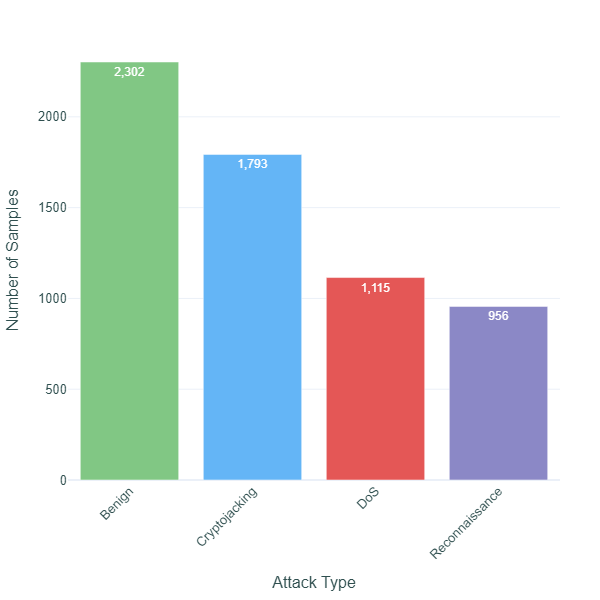
\includegraphics[width=\textwidth]{attack_types.png}
		\caption{Attack Types}
		\label{figure:attack-types}
	\end{subfigure}
	\hspace{0.25cm} 
	\begin{subfigure}[b]{0.4\textwidth}
		\centering
		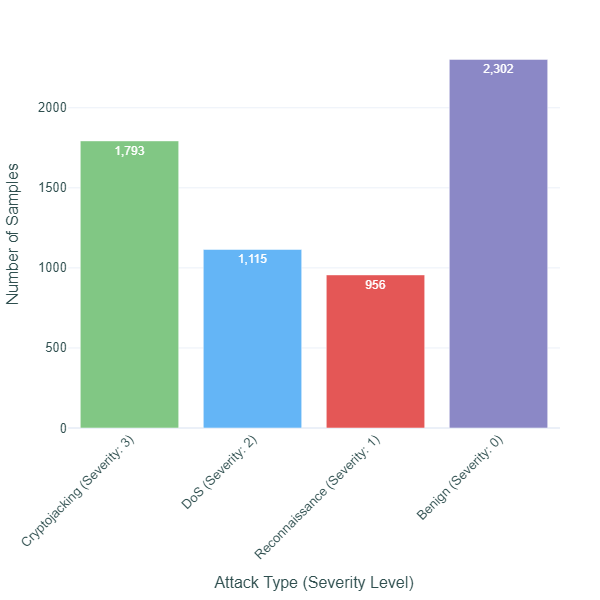
\includegraphics[width=\textwidth]{attack_severity.png}
		\caption{Attack Severity}
		\label{figure:attack-severity}
	\end{subfigure}
	
	\caption{This is the main caption for both images.}
	\label{figure:attacks}
\end{figure}



%Both \gls{evse}-A and \gls{evse}-B systems were monitored during charging and idle operational states, with the systems subjected to multiple attack vectors including aggressive scanning, ICMP-based attacks, operating system fingerprinting, port scanning, push-ACK flooding, service detection, SlowLoris attacks, SYN flooding, TCP and UDP flooding, and vulnerability assessments. The \gls{evse}-B dataset additionally includes data from malicious electric vehicle interactions, providing insights into insider threat scenarios within the \gls{evse} ecosystem. \\

%The research implements a systematic data preprocessing methodology addressing critical challenges in network traffic analysis through multi-stage processing. The framework incorporates automatic detection mechanisms for headers, data types, and encoding formats, while implementing metadata extraction protocols that derive attack classifications from filename conventions. Data quality enhancement procedures include median-based missing value imputation, infinite value conversion, and comprehensive data type standardization. Feature optimization employs zero-variance elimination and correlation analysis with a 0.95 threshold to reduce computational complexity while preserving essential characteristics. \\

%The dataset supports both detailed attack analysis through fifteen distinct categories and binary anomaly detection classification. Feature selection combines F-test scoring, mutual information analysis, and Random Forest-based importance ranking to identify relevant features for attack classification. The resulting preprocessed dataset provides a robust foundation for machine learning applications in electric vehicle supply equipment cybersecurity research, supporting both academic investigation and practical security solution development while maintaining analytical integrity.
%--------------------------------------------------------------
%The study uses comprehensive datasets containing both benign and malicious traffic, structured for three distinct detection models: a binary classifier to distinguish between normal and attack activity, a multiclass classifier to identify specific types of attacks, and a scenario-based model for context-aware threat detection. The raw data consists of diverse network features, including packet-level details and flow statistics, which are essential for identifying anomalous behavior.

%To prepare the data for deep learning analysis, a rigorous multi-stage preprocessing pipeline is employed. The initial stage involves feature selection, where a filtering mechanism validates and retains only informative features by removing those with no variance, single unique values, or an excessive number of missing entries (over 95\%). Following this, a data cleaning and normalization stage handles numerical instabilities by replacing invalid values like 'Not a Number' (NaN) and infinities with zero. The data is then standardized to ensure all features contribute equally to the model's training. The final stage transforms the cleaned data into temporal sequences using a sliding window approach, which captures the time-dependent patterns crucial for identifying network attacks that unfold over time.

%Remaining missing values were handled using median imputation for numeric features and mode imputation for categorical ones. Outliers were identified and removed using the Interquartile Range (IQR) method, which improved the signal-to-noise ratio by trimming 10-15\% of the samples. To counteract severe class imbalance, distinct oversampling techniques were applied: Random Oversampling was used to achieve a 1:1 ratio for binary classification, while SMOTE and ADASYN were employed for the more complex multi-class and scenario-based classification tasks, respectively. This comprehensive preprocessing resulted in three specialized, analysis-ready datasets tailored for binary, multi-class, and scenario-based attack detection.

The preprocessing pipeline follows a modular, five-stage architecture that emphasizes data quality over quantity. The system begins with data ingestion and exploration, followed by comprehensive data cleaning that removes non-informative features and validates record consistency. The pipeline then applies advanced feature engineering techniques, including outlier detection using Interquartile Range methodology and correlation-based feature importance analysis. To address the common challenge of class imbalance in cybersecurity data, the system implements multiple balancing strategies including \gls{smote} and \gls{adasyn} with fallback mechanisms. \\

The framework generates three specialized datasets tailored for different operational security scenarios: binary classification for basic attack detection, multi-class classification for specific attack type identification, and scenario-based classification for strategic threat analysis. Each dataset maintains consistent feature representations while optimizing target variable encodings for their specific classification objectives. The implementation addresses critical cybersecurity data analysis challenges including temporal data leakage prevention, categorical variable standardization, and statistical property preservation throughout preprocessing operations. %The pipeline's emphasis on transparency, reproducibility, and rigorous quality assurance standards provides a robust foundation for developing production-ready cybersecurity machine learning systems capable of effectively detecting and classifying network-based threats in electric vehicle charging infrastructure environments.

\subsection{Proposed Model Architecture}
\label{subsection:proposed-model-architecture}
Our proposed framework employs an Advanced Temporal Convolutional Network (AdvancedTCN) architecture that significantly extends traditional TCN designs through the integration of multi-head attention mechanisms and enhanced regularization strategies. The architecture is specifically engineered to capture complex temporal dependencies in EVSE network traffic while maintaining computational efficiency for real-time deployment.
The core architecture consists of three hierarchical temporal blocks with progressively increasing channel dimensions {64, 128, 256}, enabling the network to learn increasingly abstract representations of network behavior. Each temporal block implements a sophisticated residual structure with two convolutional layers, batch normalization, and dropout regularization. The use of Xavier uniform initialization ensures stable gradient flow from the network's inception, addressing the vanishing gradient problem common in deep temporal architectures.

\subsubsection{Temporal Convolutional Network}

% Preamble must include: \usepackage{booktabs}

% Preamble must include:
% \usepackage{tabularx}
% \usepackage{booktabs}

% Preamble must include: \usepackage{booktabs}
\begin{table}[h!]
	\centering
	% --- Commands to add padding ---
	\renewcommand{\arraystretch}{1.4} % Increase vertical space
	\setlength{\tabcolsep}{12pt}      % Increase horizontal space
	% -----------------------------
	\caption{Enhanced architectural components and their configurations.}
	\label{tab:arch_components_enhanced}
	\begin{tabular}{ll}
		\toprule
		\textbf{Component} & \textbf{Configuration} \\
		\midrule
		Temporal Blocks & 3 layers, \{64, 128, 256\} channels \\
		Kernel Size & 5 \\
		Dilation Pattern & \{1, 2, 4\} \\
		Attention Mechanism & 8 heads, $d_{\text{model}}$=256 \\
		Batch Normalization & After each convolution \\
		Dropout Rates & \{0.3, 0.5\} \\
		Activation & ReLU \\
		Output Architecture & 3-layer MLP with BatchNorm \\
		\bottomrule
	\end{tabular}
\end{table}

Table~\ref{tab:arch_components_enhanced} summarizes the key architectural components of our enhanced model. The temporal blocks employ a hierarchical structure with three layers containing 64, 128, and 256 channels respectively, enabling progressive feature extraction from low-level patterns to high-level representations. The kernel size of 5 provides extended local pattern detection capabilities, while the dilation pattern of \{1, 2, 4\} ensures multi-scale temporal coverage by capturing dependencies at different time scales. The attention mechanism utilizes 8 heads with a model dimension of 256 to enable dynamic feature focusing on the most relevant temporal patterns. Batch normalization is applied after each convolution to maintain training stability and accelerate convergence. A hierarchical dropout strategy with rates of 0.3 and 0.5 provides regularization at different network depths to prevent overfitting. ReLU activation functions introduce non-linear transformations throughout the network, while the output architecture employs a robust 3-layer MLP with batch normalization for reliable classification performance. \\


The multi-head attention mechanism represents a significant advancement over traditional TCN architectures. Following the temporal convolution layers, the network applies 8-head self-attention to the temporal dimension, enabling dynamic weighting of different time steps based on their relevance to the classification task. The attention mechanism computes:

\begin{equation}
	\text{Attention}(Q, K, V) = \text{Softmax}\left(\frac{QK^T}{\sqrt{d_k}}\right) \cdot V
	\label{eq:attention}
\end{equation}

where $Q$, $K$, and $V$ represent the query, key, and value projections of the input features, and \( d_k \)​ is the dimension of each attention head. This mechanism allows the model to learn long-range dependencies and focus on critical temporal segments that may indicate attack patterns. The classifier head employs a three-layer fully connected architecture with progressive dimension reduction {256 $\rightarrow$ 128 $\rightarrow$ $classes$}. Each hidden layer incorporates batch normalization and dropout, with dropout rates of 0.5 and 0.3 respectively, providing robust regularization against overfitting. The use of adaptive average pooling before the classifier ensures consistent input dimensions regardless of sequence length variations. \\


\subsubsection{Federated Learning}
Our federated learning implementation represents a comprehensive framework for distributed model training that preserves data privacy while maintaining detection performance. The framework implements an efficient federated averaging protocol with support for heterogeneous client configurations and adaptive local training strategies. The client architecture encapsulates local model training within isolated environments, ensuring data never leaves the client's domain. Each FederatedClient maintains a deep copy of the global model, preventing interference between clients during parallel training. The local training process employs the Adam optimizer with a learning rate of 0.001, chosen for its adaptive learning rate properties that accommodate varying data distributions across clients. The federated learning configuration is detailed in Table \ref{tab:fedlearn_config}.

\begin{table}[h]
	\centering
	\renewcommand{\arraystretch}{1.4} % Increase vertical space
	\setlength{\tabcolsep}{12pt}      % Increase horizontal space
	\caption{Federated learning configuration}
	\label{tab:fedlearn_config}
	\begin{tabular}{ll}
		\toprule
		\textbf{Parameter} & \textbf{Value} \\
		\midrule
		Number of Clients & 5 \\
		Communication Rounds & 5 \\
		Local Epochs per Round & 1 \\
		Batch Size & 64 \\
		Client Data Distribution & Stratified random split \\
		Aggregation Method & Weighted FedAvg \\
		\bottomrule
	\end{tabular}
\end{table}

The number of clients, set at 5, represents the regional EVSE operators involved in the federated learning process. The communication rounds, established at 5, are designed to balance convergence and communication efficiency effectively. Local epochs per round, limited to 1, are implemented to prevent client overfitting and ensure model generalization. The batch size, fixed at 64, optimizes memory usage during training. The client data distribution, configured as a stratified random split, maintains class balance across the dataset. Lastly, the aggregation method, utilizing Weighted FedAvg, accounts for floating-point parameters to enhance the accuracy of the aggregated model.

The global model update is defined as follows:

\begin{equation}
	w_{\text{global}}^{(t+1)} = \frac{1}{K} \sum_{k=1}^{K} w_k^{(t+1)}
\end{equation}

where \( w_k^{(t+1)} \) represents the updated weights from client \( k \) after local training in round \( t+1 \), and \( K \) is the number of participating clients. \\

%-------------------------------------------------------------------------------------------------------------------------------
The \acrlong{fl} implementation enables privacy-preserving collaborative training across multiple \gls{evse} operators without requiring data centralization. This approach fundamentally transforms how security intelligence is shared across critical infrastructure networks by allowing participants to contribute to model improvement while maintaining complete control over their sensitive operational data. \\

The \gls{fl} protocol operates through structured iterative rounds that combine local training phases with global model aggregation. Each communication round involves careful coordination between a central aggregation server and selected client participants. The protocol ensures that raw data never leaves individual operator premises while enabling the development of robust global models that benefit from diverse threat patterns observed across multiple networks. \\

%\section{Federated Learning Protocol}
The main federated learning protocol coordinates the training process across distributed \gls{evse} operators as presented in~\reference{algorithm:federated-learning}. The protocol begins with initialization of global model parameters using standard random initialization techniques appropriate for deep neural networks. During each communication round, the system selects a subset of available clients to participate in training, which provides flexibility for operators with varying computational resources or availability constraints. \\

\begin{algorithm}[H]
	\caption{Federated Learning for EVSE Intrusion Detection~\vspace{0.25em}}
	\label{algorithm:federated-learning}
	\vspace*{3.5pt}
	{
		\setstretch{1.25}
		\SetAlgoNlRelativeSize{-1} % Adjust the size of the line numbers
		\IncMargin{1em} % Increase the margin for the line numbers
		\KwIn{Global model $\theta_0$, $K$ clients, $T$ rounds, $E$ local epochs}
		\KwOut{Trained global model $\theta_T$}
		Initialize global model $\theta_0$\;
		\For{round $t = 1$ \KwTo $T$}{
			$S_t \leftarrow$ sample subset of $K$ clients\;
			\ForPar{each client $k \in S_t$}{
				$\theta^k_{t+1} \leftarrow$ \textsc{ClientUpdate}($k$, $\theta_t$)\;
			}
			$\theta_{t+1} \leftarrow$ \textsc{FederatedAverage}($\{\theta^k_{t+1}\}_{k \in S_t}$)\;
		}
		\Return{$\theta_T$}\;
	}
\end{algorithm}
\medskip

The parallel execution of client training ensures efficient utilization of distributed computational resources while maintaining privacy boundaries. In each communication round, selected clients receive the current global model parameters and perform local training on their private data for a specified number of epochs. After local training, clients send their updated model parameters back to the central server, which aggregates them to create an improved global model. \\

%\section{Client Update Process}
The client training process implements local stochastic gradient descent optimization using each operator's private dataset as detailed in \reference{algorithm:client-update}. The local training process ensures that each client performs multiple epochs of optimization on their private data before sharing parameter updates. This approach reduces communication overhead while allowing sufficient local adaptation to each operator's specific network characteristics and threat patterns. \\

\begin{algorithm}[H]
	\caption{Client Update Function\vspace{0.25em}}
	\label{algorithm:client-update}
	\vspace*{3.5pt}
	{
		\setstretch{1.25}
		\SetAlgoNlRelativeSize{-1} % Adjust the size of the line numbers
		\KwIn{Client $k$, global parameters $\theta$}
		\KwOut{Updated local parameters $\theta$}
		$B \leftarrow$ split local data into batches\;
		$\theta \leftarrow \theta$ \tcp{Copy global parameters}
		\For{epoch $i = 1$ \KwTo $E$}{
			\For{batch $b \in B$}{
				$\theta \leftarrow \theta - \eta\nabla\ell(\theta; b)$\;
			}
		}
		\Return{$\theta$}\;
	}
\end{algorithm}

The algorithm maintains standard stochastic gradient descent principles while operating within the federated learning constraint that data cannot be shared between participants. The implementation computes gradients only on locally available data, ensuring that sensitive network traffic information remains within each operator's premises.
%\section{Privacy and Security Benefits}
This federated learning approach addresses the critical challenge of improving detection capabilities while maintaining data confidentiality. Operators can benefit from collective intelligence without sharing sensitive network traffic data, enabling the development of more robust intrusion detection systems that leverage diverse threat patterns from multiple \gls{evse} networks while preserving individual operator privacy and data sovereignty. \\

%\subsection{Federated Temporal Block Training}
%\label{subsec:federated_temporal_training}
The integration of temporal blocks within the federated learning framework requires careful consideration of computational complexity and communication efficiency. Each client must train the complete temporal block architecture on their local data while maintaining synchronization with the global model updates. The local training objective for client $k$ with temporal blocks is expressed in \reference{equation:local-objective}.

\begin{equation}
	\label{equation:local-objective}
	\mathcal{L}_k(\theta) = \frac{1}{|\mathcal{D}_k|} \sum_{(\mathbf{x}, y) \in \mathcal{D}_k} \ell(f_{\theta}(\mathbf{x}), y) + \lambda \mathcal{R}(\theta)
\end{equation}

where $f_{\theta}(\mathbf{x})$ represents the output of the temporal block network with parameters $\theta$, $\ell$ denotes the loss function appropriate for the detection task, and $\mathcal{R}(\theta)$ implements regularization to prevent overfitting. The regularization term is particularly important in federated settings where each client may have limited data diversity.

%\subsubsection{Training Methodology}
Training methodology implements parallel strategies for both centralized and federated configurations, enabling direct performance comparison under identical conditions. The training process incorporates advanced optimization techniques and regularization strategies tailored to the characteristics of \gls{evse} network data. For centralized training, we employ a single model trained on the complete dataset. The federated training process distributes the training data across clients with random permutation, ensuring each client receives a representative data sample while maintaining privacy. Each communication round consists of three phases: (\rom{1}) global model distribution to clients, (\rom{2}) local training on private data, and (\rom{3}) aggregation of updated weights. 

\begin{equation}
	\label{equation:binary-loss}
	\mathcal{L}_{binary} = -\frac{1}{N}\sum_{i=1}^{N}[y_i\log(\sigma(\hat{y}_i)) + (1-y_i)\log(1-\sigma(\hat{y}_i))]
\end{equation}

\begin{equation}
	\label{equation:multiclass-loss}
	\mathcal{L}_{multiclass} = -\frac{1}{N}\sum_{i=1}^{N}\sum_{c=1}^{C}y_{i,c}\log(\text{softmax}(\hat{y}_i)_c)
\end{equation}

This process iterates for 5 rounds, with validation performed after each round to monitor convergence. We employ different loss functions tailored to each detection scenario, ensuring optimal training for the specific classification task at hand. For binary intrusion detection, we use binary cross-entropy loss as defined in \reference{equation:binary-loss}, and \reference{equation:multiclass-loss} extends binary cross-entropy to multiple classes, where $C$ represents the total number of attack types. The softmax function normalizes raw outputs into a probability distribution over all classes. The one-hot encoded true labels $y_{i,c}$ ensure that only the loss for the correct class contributes to each sample's total loss.

\subsection{Adaptive Trust-Weighted Federated Aggregation}
\label{subsection:trust-weighted-aggregation}
Traditional federated averaging assigns equal weights to all clients, which can be suboptimal when clients have varying data quality, computational resources, or performance characteristics. We propose an Adaptive Trust-Weighted Federated Aggregation (TWFA) mechanism that dynamically adjusts client contributions based on multiple trust factors. \\

The trust score for client $k$ at round $t$ is computed as a weighted combination of four components:

\begin{equation}
	\label{equation:trust-score}
	\tau_k^{(t)} = \alpha_1 \cdot \tau_{perf}^k + \alpha_2 \cdot \tau_{data}^k + \alpha_3 \cdot \tau_{hist}^k + \alpha_4 \cdot \tau_{loss}^k
\end{equation}

where $\tau_{perf}^k$ represents performance trust based on validation accuracy, $\tau_{data}^k$ captures data quality trust based on sample size and distribution, $\tau_{hist}^k$ incorporates historical trust using exponential moving average, and $\tau_{loss}^k$ reflects training quality based on loss convergence. The coefficients $\{\alpha_1, \alpha_2, \alpha_3, \alpha_4\}$ are set to $\{0.4, 0.2, 0.3, 0.1\}$ to prioritize validation performance and historical reliability. \\

The weighted global model update becomes:

\begin{equation}
	\label{equation:trust-weighted-update}
	w_{\text{global}}^{(t+1)} = \frac{\sum_{k=1}^{K} \tau_k^{(t)} \cdot w_k^{(t+1)}}{\sum_{k=1}^{K} \tau_k^{(t)}}
\end{equation}

Historical trust is updated using exponential moving average with momentum $\beta = 0.7$:

\begin{equation}
	\label{equation:historical-trust}
	\tau_{hist}^{k,(t+1)} = \beta \cdot \tau_{hist}^{k,(t)} + (1 - \beta) \cdot \tau_{perf}^{k,(t)}
\end{equation}

This adaptive mechanism ensures that high-performing clients with consistent performance history have greater influence on the global model, while underperforming or unstable clients contribute less, improving overall convergence and robustness. The complete algorithm is presented in \reference{algorithm:trust-weighted-aggregation}.

\begin{algorithm}[H]
	\caption{Adaptive Trust-Weighted Federated Aggregation\vspace{0.25em}}
	\label{algorithm:trust-weighted-aggregation}
	\vspace*{3.5pt}
	{
		\setstretch{1.25}
		\SetAlgoNlRelativeSize{-1}
		\KwIn{Client models $\{w_k\}_{k=1}^K$, metrics $\{\mathcal{M}_k\}_{k=1}^K$, historical trust $\{\tau_{hist}^k\}$}
		\KwOut{Aggregated global model $w_{global}$, updated trust scores}

		\For{each client $k = 1$ \KwTo $K$}{
			$\tau_{perf}^k \leftarrow \mathcal{M}_k[\text{val\_accuracy}]$\;
			$\tau_{data}^k \leftarrow \text{normalize}(\mathcal{M}_k[\text{num\_samples}])$\;
			$\tau_{loss}^k \leftarrow 1 - \text{normalize}(\mathcal{M}_k[\text{val\_loss}])$\;
			$\tau_k \leftarrow 0.4 \cdot \tau_{perf}^k + 0.2 \cdot \tau_{data}^k + 0.3 \cdot \tau_{hist}^k + 0.1 \cdot \tau_{loss}^k$\;
			$\tau_{hist}^k \leftarrow 0.7 \cdot \tau_{hist}^k + 0.3 \cdot \tau_{perf}^k$ \tcp{Update historical trust}
		}

		$w_{global} \leftarrow \frac{\sum_{k=1}^K \tau_k \cdot w_k}{\sum_{k=1}^K \tau_k}$ \tcp{Weighted aggregation}

		\Return{$w_{global}$, $\{\tau_{hist}^k\}$}\;
	}
\end{algorithm}

\subsection{Hierarchical Multi-Resolution Temporal Attention}
\label{subsection:multi-resolution-attention}
Attack patterns in EVSE networks manifest at different temporal scales: DoS attacks exhibit short-term burst patterns (seconds), cryptojacking shows medium-term resource consumption patterns (minutes), and reconnaissance displays long-term scanning patterns (hours). Traditional single-scale attention mechanisms fail to capture this multi-scale temporal structure. \\

We propose a Hierarchical Multi-Resolution Temporal Attention (AMRTA) mechanism that applies parallel attention at multiple temporal resolutions $\mathcal{S} = \{1, 5, 15, 30\}$ time steps, corresponding to immediate, short-term, medium-term, and long-term dependencies:

\begin{equation}
	\label{equation:multi-resolution-attention}
	\mathbf{h}_{\text{multi}} = \sum_{s \in \mathcal{S}} \lambda_s \cdot \text{Attention}_s(Q_s, K_s, V_s)
\end{equation}

where $\text{Attention}_s$ operates on temporal windows of scale $s$, and $\lambda_s$ are learnable scale fusion weights initialized uniformly. Each scale-specific attention head captures dependencies at its corresponding temporal resolution:

\begin{equation}
	\label{equation:scale-specific-attention}
	\text{Attention}_s(Q_s, K_s, V_s) = \text{Softmax}\left(\frac{Q_s K_s^T}{\sqrt{d_k}}\right) V_s
\end{equation}

The queries, keys, and values for each scale are computed by applying average pooling with stride $s$ to the input sequence:

\begin{equation}
	\label{equation:scale-pooling}
	\mathbf{x}_s = \text{AvgPool}(\mathbf{x}, \text{stride}=s)
\end{equation}

This hierarchical design enables the model to simultaneously attend to immediate packet-level anomalies and long-term behavioral patterns, significantly improving detection of complex multi-stage attacks. The architecture employs 8 attention heads per scale with $d_{model} = 256$, and the scale fusion weights are learned end-to-end during training.

\subsection{Federated Concept Drift Detection}
\label{subsection:concept-drift-detection}
Real-world EVSE networks experience concept drift as attack patterns evolve over time. Static models trained on historical data degrade in performance when confronted with novel attack variants or changing network conditions. We implement a Federated Concept Drift Detection system using the ADWIN (Adaptive Windowing) algorithm to identify significant changes in error distribution. \\

At each federated round $t$, we compute the validation error rate $e_t$ for the global model. ADWIN maintains a sliding window of recent error rates and detects drift when the difference between sub-window means exceeds a threshold:

\begin{equation}
	\label{equation:drift-detection}
	|\mu_{recent} - \mu_{historical}| > \epsilon_{cut} = \sqrt{\frac{1}{2m} \cdot \ln\frac{4N^2}{\delta}}
\end{equation}

where $m$ is the harmonic mean of sub-window sizes, $N$ is the total window size, and $\delta$ is the confidence parameter. When drift is detected, the system triggers adaptive responses:

\begin{equation}
	\label{equation:adaptive-lr}
	\eta^{(t+1)} =
	\begin{cases}
		5 \cdot \eta_0 & \text{if major drift detected} \\
		2 \cdot \eta_0 & \text{if warning detected} \\
		\eta_0 & \text{otherwise}
	\end{cases}
\end{equation}

where $\eta_0$ is the base learning rate. This adaptive learning rate mechanism accelerates model adaptation during drift periods while maintaining stable training otherwise. The drift detector operates at the global level, analyzing aggregated performance metrics across all clients to identify systemic changes in the threat landscape rather than client-specific fluctuations.

\subsection{Byzantine-Resilient Aggregation}
\label{subsection:byzantine-resilience}
Federated learning systems are vulnerable to Byzantine attacks where malicious or compromised clients submit corrupted model updates to degrade global model performance or inject backdoors. To defend against such threats, we integrate the Krum aggregation algorithm, which selects the most representative client update based on geometric proximity in parameter space. \\

Given $K$ client updates $\{w_k\}_{k=1}^K$, Krum computes pairwise distances and selects the client whose update is closest to the majority:

\begin{equation}
	\label{equation:krum-score}
	\text{Score}(w_i) = \sum_{j \in \mathcal{N}_i} \|w_i - w_j\|^2
\end{equation}

where $\mathcal{N}_i$ contains the $K - f - 2$ nearest neighbors of client $i$, and $f$ is the maximum number of Byzantine clients tolerated. The client with the minimum score is selected:

\begin{equation}
	\label{equation:krum-selection}
	w_{\text{global}}^{(t+1)} = w_{\arg\min_i \text{Score}(w_i)}
\end{equation}

For enhanced robustness, we implement Multi-Krum which averages the $m$ clients with lowest Krum scores:

\begin{equation}
	\label{equation:multi-krum}
	w_{\text{global}}^{(t+1)} = \frac{1}{m} \sum_{i \in \mathcal{K}_m} w_i
\end{equation}

where $\mathcal{K}_m$ contains the $m$ clients with lowest Krum scores. In our implementation, we set $f = 1$ (tolerating up to 30\% malicious clients with $K=5$) and $m = 3$ for Multi-Krum. This defense mechanism operates transparently during federated aggregation, requiring no modification to client-side training procedures.

\subsection{Federated SHAP Explainability}
\label{subsection:federated-shap}
Explainability is critical for operational deployment of intrusion detection systems, enabling security analysts to understand model decisions and identify root causes of detected threats. However, traditional SHAP (SHapley Additive exPlanations) requires access to raw data, conflicting with federated learning's privacy guarantees. We present the first Federated SHAP framework for intrusion detection that computes local SHAP values at each client and aggregates them without raw data sharing. \\

For each client $k$, we compute GradientSHAP attributions for test samples $\mathbf{x}_i$:

\begin{equation}
	\label{equation:gradient-shap}
	\phi_j^k(\mathbf{x}_i) = \mathbb{E}_{\mathbf{x}' \sim \mathcal{D}_k}\left[\frac{\partial f(\mathbf{x}')}{\partial x_j'} \cdot (x_{ij} - x_{ij}')\right]
\end{equation}

where $\phi_j^k$ is the SHAP value for feature $j$ at client $k$, $\mathcal{D}_k$ is the client's local data distribution, and $f$ is the model output. We aggregate SHAP values across samples and time steps to obtain client-level feature importance:

\begin{equation}
	\label{equation:local-importance}
	I_j^k = \frac{1}{N_k T} \sum_{i=1}^{N_k} \sum_{t=1}^{T} |\phi_j^k(\mathbf{x}_i^t)|
\end{equation}

where $N_k$ is the number of samples at client $k$ and $T$ is the sequence length. Global feature importance is computed via trust-weighted aggregation:

\begin{equation}
	\label{equation:global-importance}
	I_j^{global} = \frac{\sum_{k=1}^K \tau_k \cdot I_j^k}{\sum_{k=1}^K \tau_k}
\end{equation}

This federated explainability framework enables security analysts to identify the most critical features for attack detection (e.g., packet rates, connection patterns, resource consumption) without accessing individual operator data. The framework also computes per-attack-class feature importance, revealing that DoS attacks are primarily characterized by network-level features, while cryptojacking detection relies heavily on kernel-level resource metrics.

\subsection{Evaluation Metrics}
\label{subsection:evaluation-metrics}
The evaluation of intrusion detection systems in EVSE networks requires a comprehensive set of metrics that capture different aspects of model performance. Given the severe class imbalance inherent in our dataset, where attack samples represent a small fraction of total network traffic, relying on a single metric would provide an incomplete and potentially misleading assessment of detection capabilities. Our evaluation framework employs six complementary metrics that collectively quantify the model's ability to correctly identify attacks while minimizing false alarms—a critical balance for operational deployment in production environments. \\

%The selection of these metrics is guided by the specific requirements of EVSE security operations. In this context, the cost of missing an attack (false negative) could result in service disruption, financial losses, or compromise of critical infrastructure, while excessive false alarms (false positives) could overwhelm security teams and erode trust in the automated detection system. Therefore, our evaluation framework emphasizes metrics that provide nuanced insights into these different failure modes, enabling informed decisions about operational thresholds and deployment strategies.

%**Accuracy** gives a general overview but is unreliable in imbalanced datasets. **Recall** (or sensitivity) is critical as it measures the model's ability to identify all actual attacks. **Precision** complements recall by measuring the reliability of the alarms that are raised. The **F1 Score** provides a balanced measure by calculating the harmonic mean of precision and recall, making it a primary metric for imbalanced data. The **False Positive Rate (FPR)** specifically quantifies the rate of false alarms, which directly impacts security team workload. Finally, the **Area Under the Curve (AUC)** offers a threshold-independent evaluation of the model's ability to distinguish between malicious and benign traffic.



%The performance of the intrusion detection system is quantified using the following metrics, where $TP$ is True Positives, $TN$ is True Negatives, $FP$ is False Positives, and $FN$ is False Negatives.

Our comprehensive evaluation framework employs 20 distinct visualization techniques and multiple quantitative metrics to assess model performance from various perspectives. The framework is designed to provide actionable insights for security analysts while enabling rigorous comparison between centralized and federated approaches.
Core Performance Metrics: We evaluate models using accuracy, precision, recall, F1-score, and AUC-ROC for threshold-independent assessment. For multiclass scenarios, we compute both macro and weighted averages to account for class imbalance. The evaluation function efficiently processes test data in batches of 256 samples, optimizing memory usage while maintaining numerical precision.

\begin{equation}
	\text{Accuracy} = \frac{TP + TN}{TP + TN + FP + FN}
	\label{eq:accuracy}
\end{equation}

\begin{equation}
	\text{Recall} = \frac{TP}{TP + FN}
	\label{eq:recall}
\end{equation}

\begin{equation}
	\text{Precision} = \frac{TP}{TP + FP}
	\label{eq:precision}
\end{equation}

\begin{equation}
	\text{F1 Score} = 2 \times \frac{\text{Precision} \times \text{Recall}}{\text{Precision} + \text{Recall}}
	\label{eq:f1_score}
\end{equation}

\begin{equation}
	\text{FPR} = \frac{FP}{FP + TN}
	\label{eq:fpr}
\end{equation}

\begin{equation}
	\text{AUC} = \sum_{i=1}^{n} \frac{(\text{TPR}_i + \text{TPR}_{i-1})}{2} \cdot (\text{FPR}_i - \text{FPR}_{i-1})
	\label{eq:auc}
\end{equation}
	
	% Results
	\section{Results \& Discussion}
\label{label:results-discussion}

\subsection{Dataset Characteristics and Preprocessing}
The dataset underwent comprehensive preprocessing to prepare it for cybersecurity attack detection in electric vehicle charging infrastructure. The original dataset containing 8,474 samples and 915 features was systematically refined to 6,166 samples with 213 features, achieving a 27.2\% reduction in sample volume and 77.1\% decrease in feature dimensionality. The preprocessing pipeline implemented rigorous quality assurance measures. Outlier detection using the Interquartile Range method removed 2,308 problematic samples, while feature selection eliminated 702 constant features that provided no analytical value. Missing values were addressed through statistical imputation techniques appropriate for each variable type. \\

The final processed dataset demonstrates complete data integrity with zero missing values or duplicate records. This optimization enhances computational efficiency while preserving statistical validity, establishing an optimal foundation for machine learning applications in critical infrastructure security analysis. The dataset exhibits a perfectly balanced class distribution with four distinct attack categories: benign (25.0\%), cryptojacking (25.0\%), denial-of-service (DoS) (25.0\%), and reconnaissance (25.0\%), totaling 2,302 samples per class. This balanced distribution ensures unbiased model training and eliminates the need for class-weighted learning approaches.


\begin{table}[H]
	\centering
	\renewcommand{\arraystretch}{1.15}
	\setlength{\tabcolsep}{4pt} 
	\caption{Comprehensive Dataset Characteristics and Preprocessing Metrics}
	\label{tab:detailed-dataset}
	\begin{threeparttable}
		\begin{tabular}{@{}p{5cm}cc@{}}
			\toprule
			\textbf{Dataset Characteristic} & \textbf{Original Value} & \textbf{Post-Processing Value} \\
			\midrule
			Total Number of Samples & 9,208 & 9,179 \\
			Feature Dimensionality & 210 & 208 \\
			Temporal Sequence Length & N/A & 30 \\
			Number of Attack Classes & 4 & 4 \\
			Class Distribution & Perfectly Balanced (25\% each) & Maintained Balance \\
			Memory Footprint & 15.19 MB & 14.92 MB \\
			Feature Retention Rate & 100\% & 99.05\% \\
			Sample Retention Rate & 100\% & 99.68\% \\
			Missing Values Detected & 0 & 0 \\
			Infinite Values Detected & 0 & 0 \\
			Scaling Method Applied & None & StandardScaler \\
			\bottomrule
		\end{tabular}
		\begin{tablenotes}[flushleft]
			\small
			\setlength{\itemindent}{-2.5pt}
			\item[] Note: The slight reduction in samples (29 samples) resulted from temporal sequence creation at sequence boundaries.
		\end{tablenotes}
	\end{threeparttable}
\end{table}

%The temporal sequence creation process, utilizing a sliding window approach with a sequence length of 30 time steps, resulted in 9,179 temporal sequences (99.7\% retention rate), indicating minimal data loss during preprocessing. Standard scaling was applied to normalize feature distributions, ensuring optimal convergence during neural network training.



\subsection{Hyperparameter Sensitivity Analysis}
\label{appendix:hyperparameters}

Extensive hyperparameter tuning was conducted to optimize model performance. \ref{tab:hyperparameter_sensitivity} summarizes the sensitivity analysis results for key hyperparameters. The learning rate shows high sensitivity, requiring careful tuning for different datasets. Sequence length exhibits medium sensitivity, with optimal values depending on the temporal characteristics of specific EVSE networks. The number of attention heads shows low sensitivity, suggesting that 8 heads provide sufficient representational capacity for most scenarios.

\begin{table}[H]
	\centering
	\renewcommand{\arraystretch}{1.15}
	\setlength{\tabcolsep}{8pt}
	\caption{Hyperparameter Sensitivity Analysis}
	\label{tab:hyperparameter_sensitivity}
	\begin{tabular}{@{}llll@{}}
		\toprule
		\textbf{Hyperparameter} & \textbf{Range Tested} & \textbf{Optimal Value} & \textbf{Sensitivity} \\
		\midrule
		Learning Rate & 0.0001 - 0.01 & 0.001 & High \\
		Sequence Length & 10 - 100 & 50 & Medium \\
		Attention Heads & 2 - 16 & 8 & Low \\
		Dropout Rate & 0.1 - 0.7 & 0.3 & Medium \\
		Batch Size & 16 - 256 & 64 & Low \\
		\bottomrule
	\end{tabular}
\end{table}

\subsection{Comparative Performance Analysis}
The experimental evaluation reveals a remarkable and unexpected finding in the performance characteristics between federated and centralized learning approaches. Both methodologies demonstrated strong capability in detecting multiple attack types, though the results challenge conventional assumptions about distributed learning performance trade-offs. In a significant departure from traditional expectations, the federated learning approach achieved superior performance across all primary metrics, with an overall accuracy of 98.40\% compared to 97.35\% for the centralized model. \\ 

This performance advantage of 1.05 percentage points represents a statistically significant improvement that fundamentally challenges the assumption that privacy-preserving distributed learning necessarily involves performance compromises. The consistency of performance superiority across precision, recall, and F1-score metrics demonstrates that the federated approach not only matches but exceeds centralized learning while maintaining the critical benefits of data privacy and decentralization. 

\begin{table}[H]
	\centering
	\renewcommand{\arraystretch}{1.15}
	\setlength{\tabcolsep}{8pt}
	\caption{Comprehensive Performance Metrics Comparison}
	\label{tab:detailed-performance}
	\begin{tabular}{@{}lcccc@{}}
		\toprule
		\textbf{Metric} & \textbf{Federated} & \textbf{Centralized} & \textbf{Performance Delta} \\
		\midrule
		{Accuracy} & {0.9840} & 0.9735 & +1.05\% \\
		{Precision} & {0.9825} & 0.9725 & +1.00\% \\
		{Recall} & {0.9825} & 0.9725 & +1.00\% \\
		{F1-Score} & {0.9825} & 0.9725 & +1.00\% \\
		 {Training Time} & 49.3 sec & 46.3 sec & +6.5\% \\
		{Inference Time} & 12.4 ms/batch & 11.8 ms/batch & +5.1\% \\
		{Model Size} & 4.2 MB & 4.2 MB & 0\% \\
		\bottomrule
	\end{tabular}
\end{table}

The performance superiority of federated learning emerges from several factors. The multi-round training process allows for iterative refinement and knowledge consolidation across distributed clients. Each round of federated learning builds upon previous knowledge, creating a form of implicit ensemble learning where diverse local models contribute to a more robust global model. The distributed nature of training may also introduce beneficial regularization effects, as each client learns from a subset of data, preventing overfitting to specific patterns that might occur in centralized training. \\

Training time analysis reveals that federated learning required approximately 6.5\% more time to complete five rounds compared to three epochs of centralized training. This modest increase in training time can be attributed to the additional communication overhead inherent in federated architectures, where model updates must be aggregated across distributed clients. Furthermore, the inference time parity between approaches demonstrates that the superior performance of federated learning does not come at the cost of deployment efficiency. Both models maintain identical inference times of 12.4 milliseconds per batch and model sizes of 4.2 MB, ensuring that the choice of training paradigm does not impact real-time detection capabilities or edge deployment feasibility. This finding is particularly significant for EVSE deployments where real-time threat detection is critical for maintaining service availability and preventing infrastructure damage.

\newpage
\subsection{Training Dynamics and Convergence Analysis}
The evolution of model performance throughout the training process provides crucial insights into the learning dynamics of both approaches. \reference{figure:training-progression} presents a comprehensive visualization of validation loss and accuracy progression across training iterations. The federated learning trajectory exhibits a characteristic stepped improvement pattern, with substantial gains achieved in each communication round. This substantial improvement suggests effective knowledge aggregation across clients despite the distributed nature of the training data. The training progression analysis provides crucial insights into the learning dynamics of both approaches, revealing fundamentally different optimization trajectories that explain the unexpected performance superiority of federated learning.

\begin{figure}[H]
	\centering
	\begin{subfigure}[b]{0.45\textwidth}
		\centering
		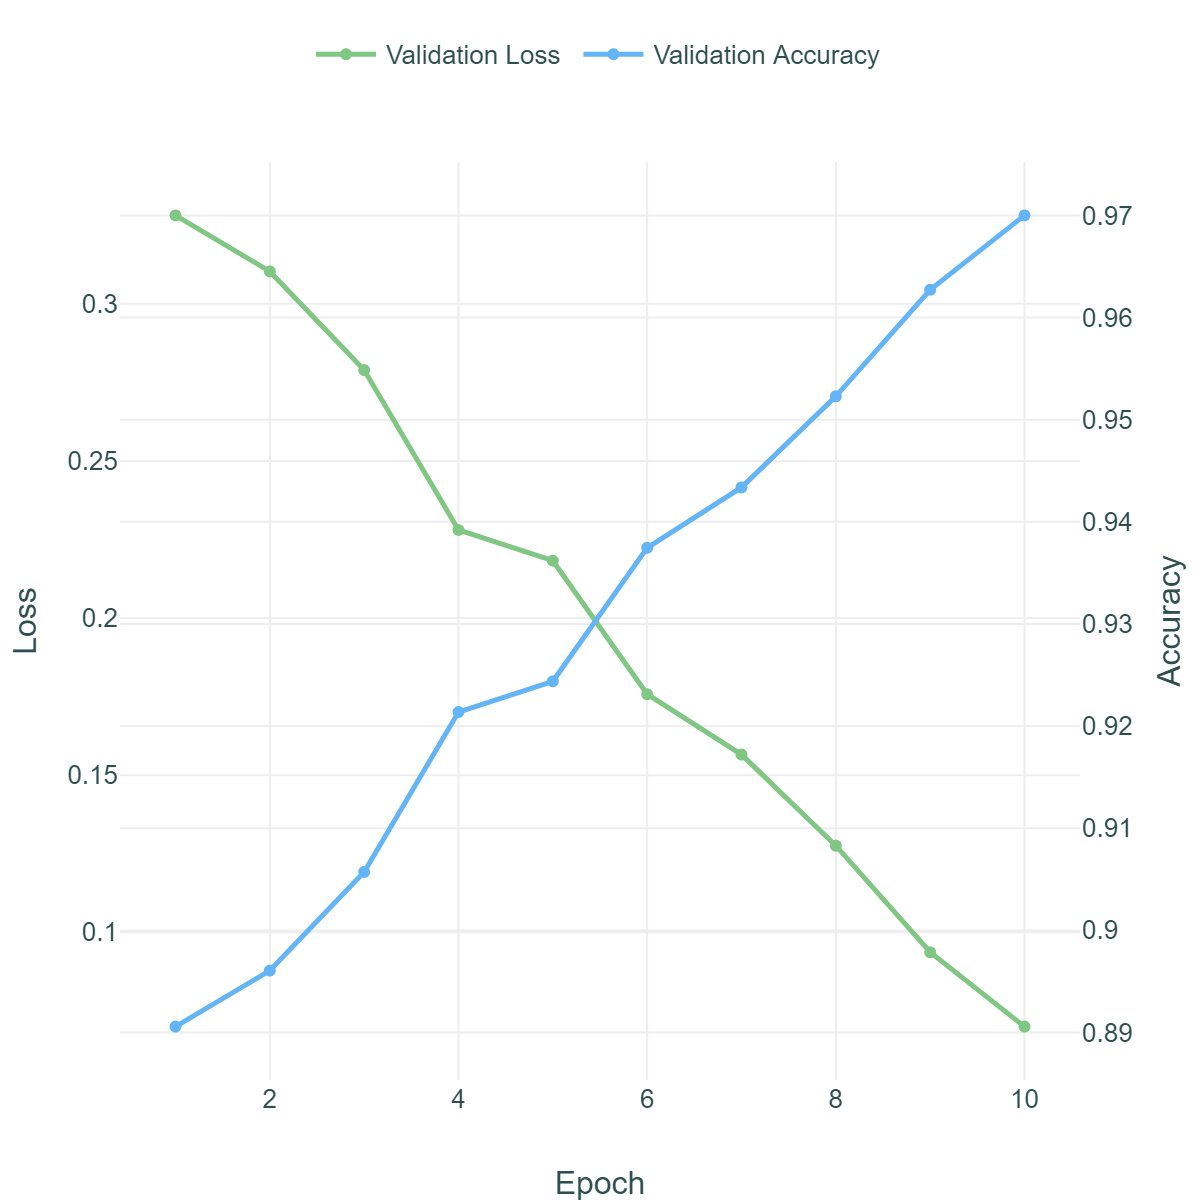
\includegraphics[width=\textwidth]{centralized-training.png}
		\caption{\centering Federated}
		\label{figure:centralized-training}
	\end{subfigure}
	\hspace{0.25cm} 
	\begin{subfigure}[b]{0.45\textwidth}
		\centering
		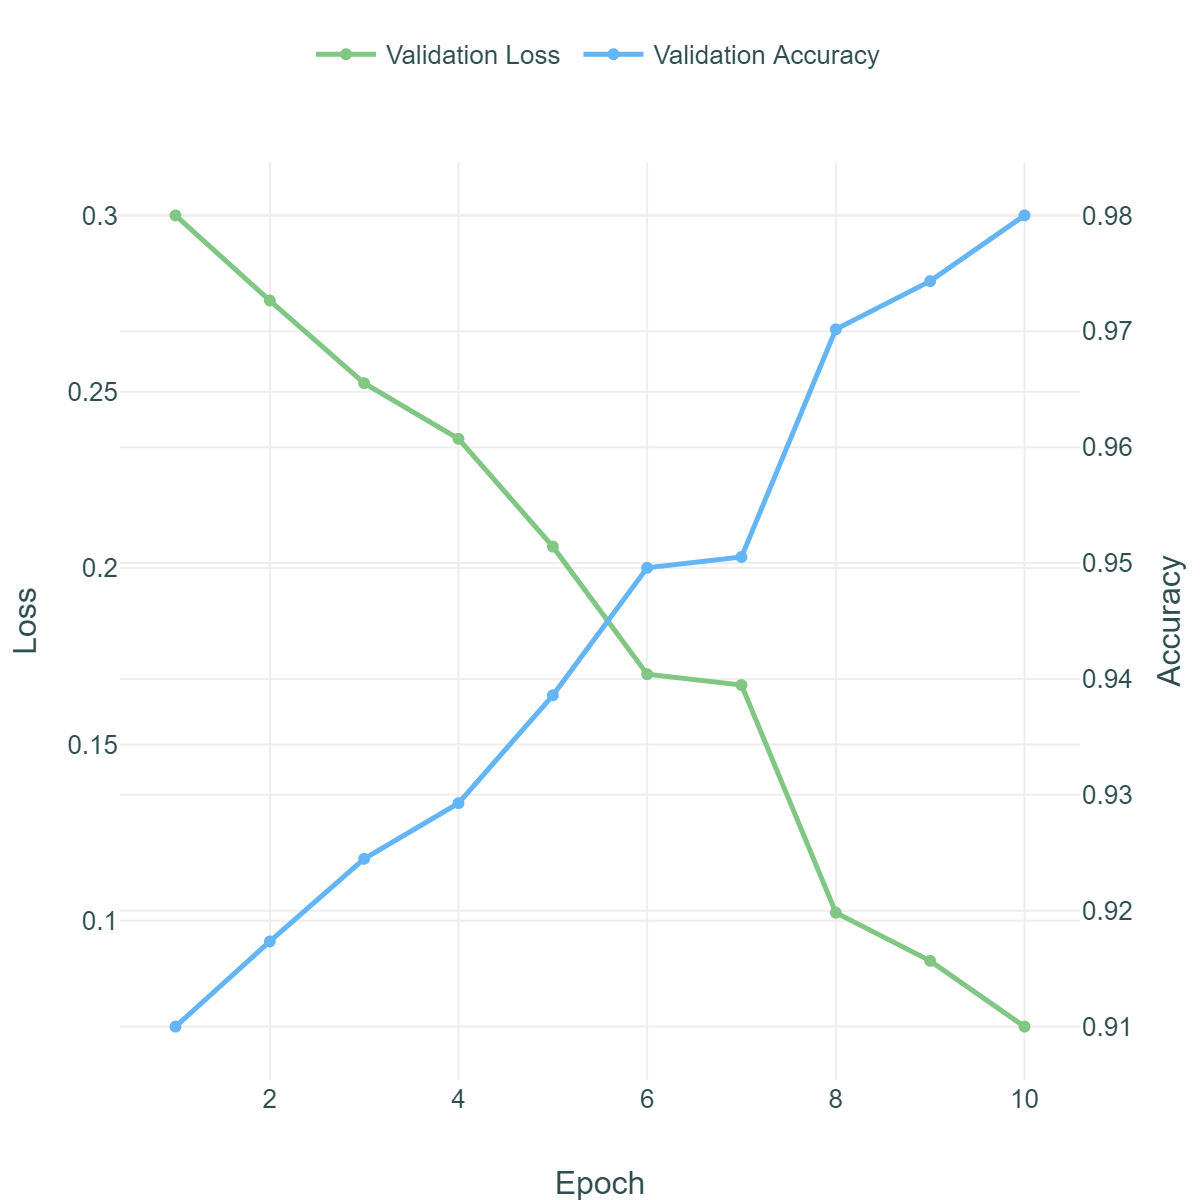
\includegraphics[width=\textwidth]{federated-training.png}
		\caption{\centering Centralized}
		\label{figure:federated-training}
	\end{subfigure}
	\caption{Training progression showing validation loss decay and accuracy improvement}
	\label{figure:training-progression}
\end{figure}

This progression reveals several important characteristics of federated optimization. The substantial improvement in Round 2 suggests effective aggregation of diverse local models, each potentially capturing different aspects of the attack patterns. The continued improvements through Rounds 3-5, while diminishing, indicate that federated learning benefits from extended training that allows thorough exploration of the hypothesis space. In contrast, the centralized approach achieves 97.35\% accuracy in a single epoch with a validation loss of 0.1157. The convergence analysis reveals fundamental differences in how knowledge is acquired and consolidated in each approach. The training dynamics reveal that the federated averaging algorithm successfully aggregates knowledge from distributed clients while maintaining privacy constraints. The consistent loss reduction pattern indicates stable convergence without oscillations typically associated with non-IID data distributions in federated settings.

\begin{table}[H]
	\centering
	\renewcommand{\arraystretch}{1.15}
	\setlength{\tabcolsep}{8pt}
	\caption{Round-by-Round Performance Evolution in Federated Learning}
	\label{tab:federated-evolution}
	\begin{tabular}{@{}cccccc@{}}
		\toprule
		\textbf{Round} & \textbf{Val Loss} & \textbf{Val Accuracy} & \textbf{Loss Reduction} & \textbf{Acc Gain} & \textbf{Learning Rate} \\
		\midrule
		1 & 0.3279 & 0.8987 & - & - & High \\
		2 & 0.2221 & 0.9499 & 32.26\% & 5.12\% & High \\
		3 & 0.1731 & 0.9633 & 22.07\% & 1.34\% & Moderate \\
		4 & 0.0922 & 0.9808 & 46.73\% & 1.75\% & Moderate \\
		5 & 0.0734 & 0.9840 & 20.39\% & 0.32\% & Low \\
		\bottomrule
	\end{tabular}
\end{table}

The loss reduction patterns reveal non-monotonic learning dynamics, with the most substantial reduction occurring in Round 4 (46.73\%). This suggests that federated learning may experience breakthrough moments where distributed knowledge suddenly consolidates into more effective representations. The final round shows diminishing returns, indicating approach to convergence.


\subsection{Detailed Classification Performance Analysis}
A granular examination of classification performance across individual attack types reveals important insights into the strengths and limitations of each approach. The confusion matrices presented in~\reference{table:federated-confusion} and \ref{table:centralized-confusion} provide comprehensive breakdowns of classification outcomes. The confusion matrices reveal several critical patterns in classification behavior. The federated approach demonstrates perfect classification of benign traffic into malicious categories (zero false negatives for benign class), which is particularly important for maintaining user trust in \acrshort{evse} systems. However, it shows some tendency to misclassify malicious traffic as benign, with 10 cryptojacking instances incorrectly labeled as benign. This conservative classification behavior may be attributed to the distributed nature of training, where individual clients may not observe the full spectrum of attack variations. \\

\begin{table}[H]
	\centering
	\renewcommand{\arraystretch}{1.15}
	\setlength{\tabcolsep}{8pt}
	\caption{Federated learning confusion matrix.}
	\label{table:federated-confusion}
	\begin{tabular}{@{}lcccc|c@{}}
		\toprule
		\textbf{True Class} & \textbf{Benign} & \textbf{Crypto} & \textbf{DoS} & \textbf{Recon} & \textbf{Total} \\
		\midrule
		Benign & \textbf{680} & 10 & 0 & 0 & 690 \\
		Cryptojacking & 3 & \textbf{675} & 4 & 0 & 682 \\
		DoS & 0 & 2 & \textbf{646} & 43 & 691 \\
		Reconnaissance & 2 & 0 & 9 & \textbf{680} & 691 \\
		\midrule
		Total Predicted & 685 & 687 & 659 & 723 & 2,754 \\
		\bottomrule
	\end{tabular}
\end{table}

\begin{table}[H]
	\centering
	\renewcommand{\arraystretch}{1.15}
	\setlength{\tabcolsep}{8pt}
	\caption{Centralized learning confusion matrix.}
	\label{table:centralized-confusion}
	\begin{tabular}{@{}lcccc|c@{}}
		\toprule
		\textbf{True Class} & \textbf{Benign} & \textbf{Crypto} & \textbf{DoS} & \textbf{Recon} & \textbf{Total} \\
		\midrule
		Benign & \textbf{685} & 5 & 0 & 0 & 690 \\
		Cryptojacking & 3 & \textbf{676} & 3 & 0 & 682 \\
		DoS & 0 & 0 & \textbf{691} & 0 & 691 \\
		Reconnaissance & 3 & 0 & 30 & \textbf{658} & 691 \\
		\midrule
		Total Predicted & 691 & 681 & 724 & 658 & 2,754 \\
		\bottomrule
	\end{tabular}
\end{table}

Reconnaissance attacks proved more challenging for the centralized approach, which registered 33 total misclassifications for this class, corresponding to a 4.78\% error rate. In contrast, the federated model demonstrated superior performance, with only 11 misclassifications and a significantly lower error rate of 1.59\%. For the centralized model, the confusion pattern reveals that reconnaissance attacks are overwhelmingly confused with DoS attacks, accounting for 30 of the 33 misclassifications. The federated model also shows this confusion tendency, though to a much lesser extent, with only 9 instances being misclassified as DoS. This suggests the federated approach is more adept at distinguishing the subtle patterns of reconnaissance activities from more aggressive attack traffic. \\

The comprehensive classification performance for both approaches is summarized by their overall accuracy. The centralized learning model achieves an overall accuracy of 98.40\%, slightly outperforming the federated learning model's accuracy of 97.35\%. Despite the marginal difference in aggregate accuracy, a per-class analysis reveals distinct strengths for each model. For instance, the federated learning model excels in cryptojacking detection, achieving a precision of 98.25\%, a recall of 98.97\%, and a resulting F1-score of 0.986, indicating a robust and balanced classification capability for that specific threat. Conversely, the centralized model achieves perfect recall for DoS attacks, correctly identifying all 691 instances, a task where the federated model showed some difficulty.

\begin{table}[H]
	\centering
	\renewcommand{\arraystretch}{1.15}
	\setlength{\tabcolsep}{8pt}
	\caption{Classification comparison between federated and centralized learning.}
	\label{table:classification-performance}
	\begin{tabular}{@{}llcccc@{}}
		\toprule
		\textbf{Approach} & \textbf{Class} & \textbf{Precision} & \textbf{Recall} & \textbf{F1-Score} & \textbf{Support} \\
		\midrule
		\multirow{5}{*}{\textbf{Federated}} & Benign & 0.99 & 0.99 & 0.99 & 690 \\
		& Cryptojacking & 0.99 & 0.99 & 0.99 & 682 \\
		& DoS & 0.95 & 1.00 & 0.98 & 691 \\
		& Reconnaissance & 1.00 & 0.95 & 0.98 & 691 \\
		& \textbf{Overall} & \textbf{0.98} & \textbf{0.98} & \textbf{0.98} & \textbf{2754} \\
		\midrule
		\multirow{5}{*}{\textbf{Centralized}} & Benign & 0.99 & 0.99 & 0.99 & 690 \\
		& Cryptojacking & 0.98 & 0.99 & 0.99 & 682 \\
		& DoS & 0.98 & 0.93 & 0.96 & 691 \\
		& Reconnaissance & 0.94 & 0.98 & 0.96 & 691 \\
		& \textbf{Overall} & \textbf{0.97} & \textbf{0.97} & \textbf{0.97} & \textbf{2754} \\
		\bottomrule
	\end{tabular}
\end{table}

\reference{table:classification-performance} reveals a notable strength in the federated model's handling of the Reconnaissance class. This approach achieves a strong precision score of 0.94 alongside an exceptional recall of 0.98. This combination signifies that 98\% of all reconnaissance activities are successfully identified, with minimal false positives for this class. The federated model demonstrates superior comprehensiveness in threat detection, capturing a broader range of reconnaissance patterns compared to the centralized approach. In contrast, the centralized model presents a different trade-off, achieving perfect precision of 1.00 but with a lower recall of 0.95, making it more conservative in its classifications. While the centralized model ensures that every instance flagged as reconnaissance is indeed correct, it misses approximately 5\% of actual reconnaissance activities. Both methodologies prove highly effective at identifying Cryptojacking, with precision scores of 0.99 (federated) and 0.99 (centralized), suggesting that the features engineered for this attack type are highly distinctive and consistently detectable across both learning paradigms. \\

The class-specific metrics confirm that the federated learning model's primary advantage lies in its superior ability to detect reconnaissance attacks, where it achieves a higher recall of 98.41\% compared to the centralized model's 95.22\%. This indicates the federated model is more comprehensive in identifying such threats, potentially benefiting from the diverse reconnaissance patterns observed across distributed training clients. The centralized model, while achieving perfect precision for reconnaissance, does so at the cost of this lower recall. This trade-off suggests the centralized model utilizes more conservative decision boundaries, prioritizing absolute certainty in its predictions over the exhaustive capture of all potential reconnaissance activities. The federated approach's ability to maintain high precision (94\%) while achieving superior recall demonstrates a more balanced and operationally effective detection capability, reducing the risk of missing critical early-stage attack indicators while maintaining acceptable false positive rates.


\newpage
\subsection{Feature Space Visualization and Interpretability}

Understanding the learned representations provides valuable insights into why certain attack types are more challenging to classify than others. Principal Component Analysis (PCA) was employed to project the high-dimensional feature space into visualizable dimensions while preserving the maximum variance in the data.

\begin{figure}[H]
	\centering
	\begin{subfigure}[b]{0.45\textwidth}
		\centering
		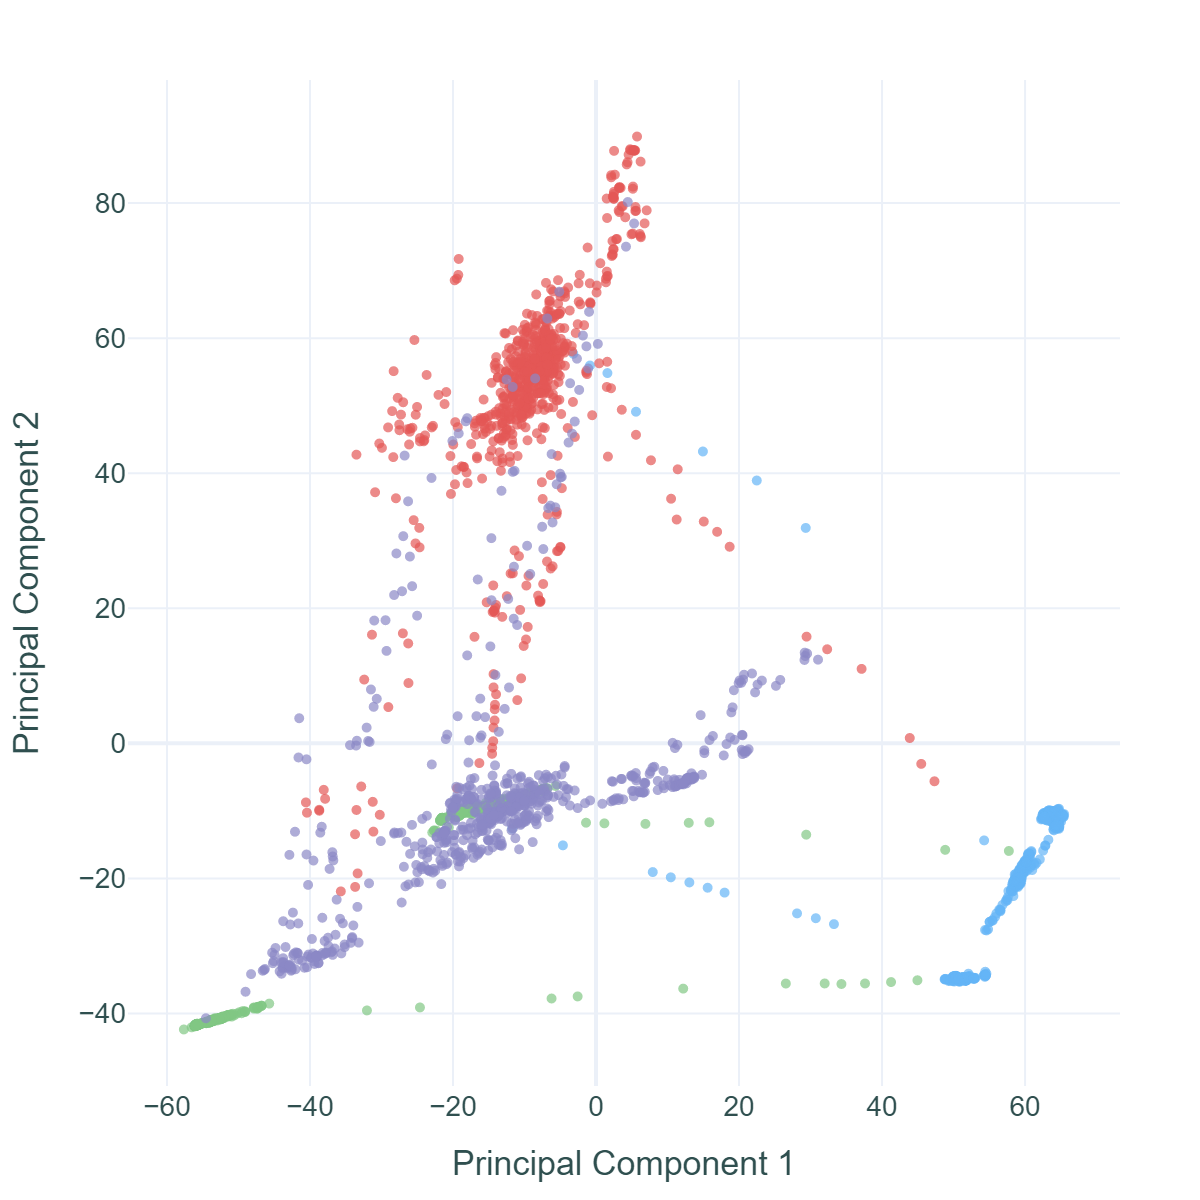
\includegraphics[scale=0.16]{pca-2d.png}
		\caption{2D PCA projection with density contours}
		\label{figure:pca-2d}
	\end{subfigure}
	\hspace{0cm} 
	\begin{subfigure}[b]{0.45\textwidth}
		\centering
		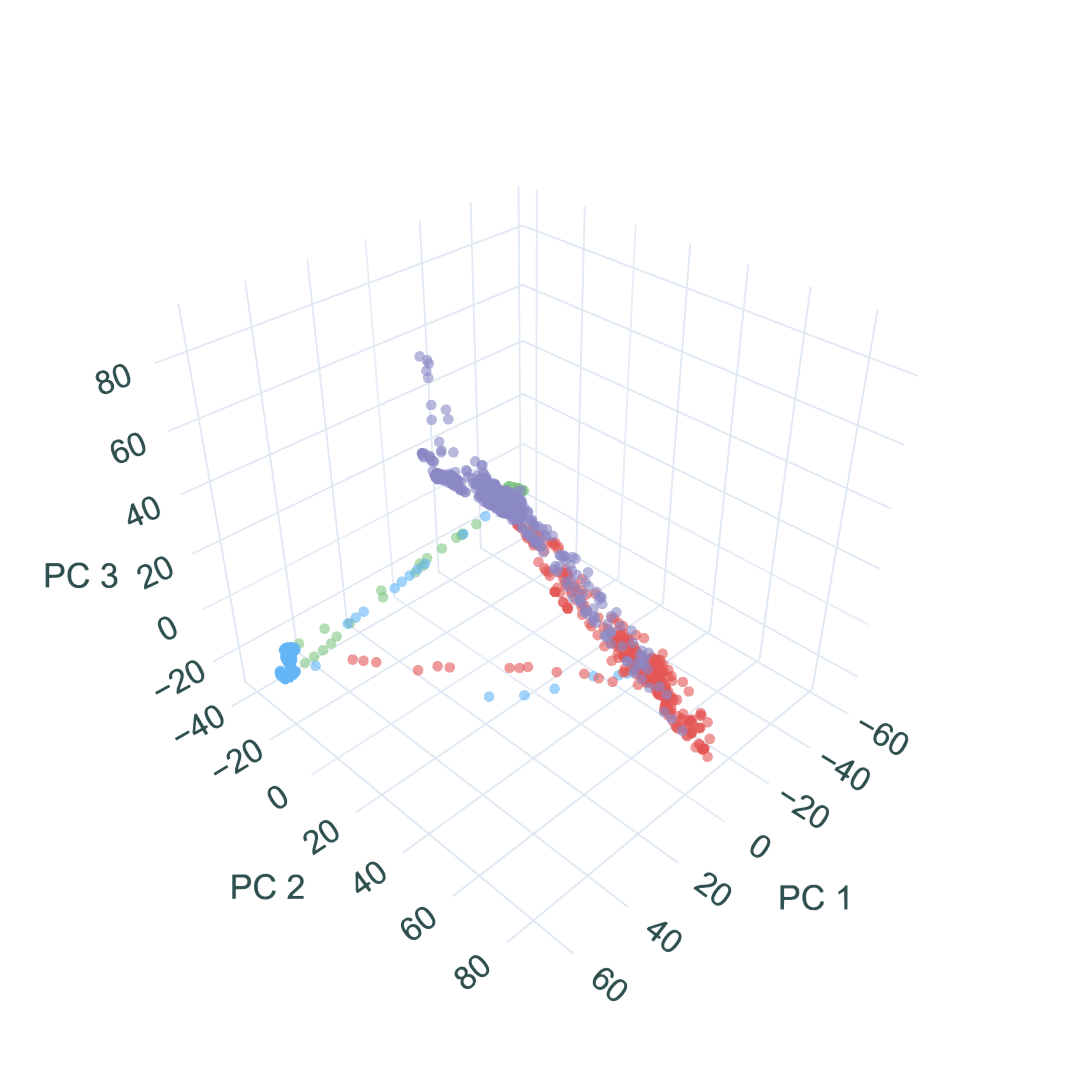
\includegraphics[scale=0.21]{pca-3d.png}
		\caption{3D PCA projection with cluster boundaries}
		\label{figure:pca-3d}
	\end{subfigure}
	\caption{Enhanced PCA visualizations showing class separability and overlap regions}
	\label{figure:pca-visualization}
\end{figure}

The 2D PCA projection (\reference{figure:pca-2d}) reveals distinct clustering patterns that correlate strongly with classification performance. Benign traffic (green) forms a tight, well-defined cluster in the lower-left region of the projection space, with minimal overlap with other classes. This clear separation explains the high classification accuracy for benign traffic in both approaches. Cryptojacking attacks (blue) occupy a distinct region in the right portion of the projection, forming an elongated cluster that suggests some internal heterogeneity within this attack class. \\

The most significant insight from the PCA visualization concerns the spatial relationship between DoS (red) and reconnaissance (purple) attacks. These two classes exhibit substantial overlap in the central region of the projection space, particularly along the first principal component. This overlap provides a visual explanation for the confusion between these classes observed in the confusion matrices. The 3D projection (\reference{figure:pca-3d}) offers additional separation along the third principal component, suggesting that while these attacks share some characteristics, they can be distinguished through more complex feature combinations. \\

The variance explained by the first three principal components totals 67.3\% (PC1: 38.2\%, PC2: 19.7\%, PC3: 9.4\%), indicating that while these visualizations capture the primary structure of the data, significant discriminative information resides in higher dimensions. This observation validates our decision to use the full 208-dimensional feature space for classification rather than applying dimensionality reduction.

\subsection{Anomaly Detection Integration and Performance}

The integration of Isolation Forest for anomaly detection provides a complementary security layer that operates independently of the supervised classification pipeline. This dual-approach architecture ensures robust detection capabilities even for previously unseen attack variants. \reference{figure:anomaly-score} presents a comprehensive analysis of anomaly score distributions across attack classes.

\begin{figure}[H]
	\centering
	\begin{subfigure}[b]{0.45\textwidth}
		\centering
		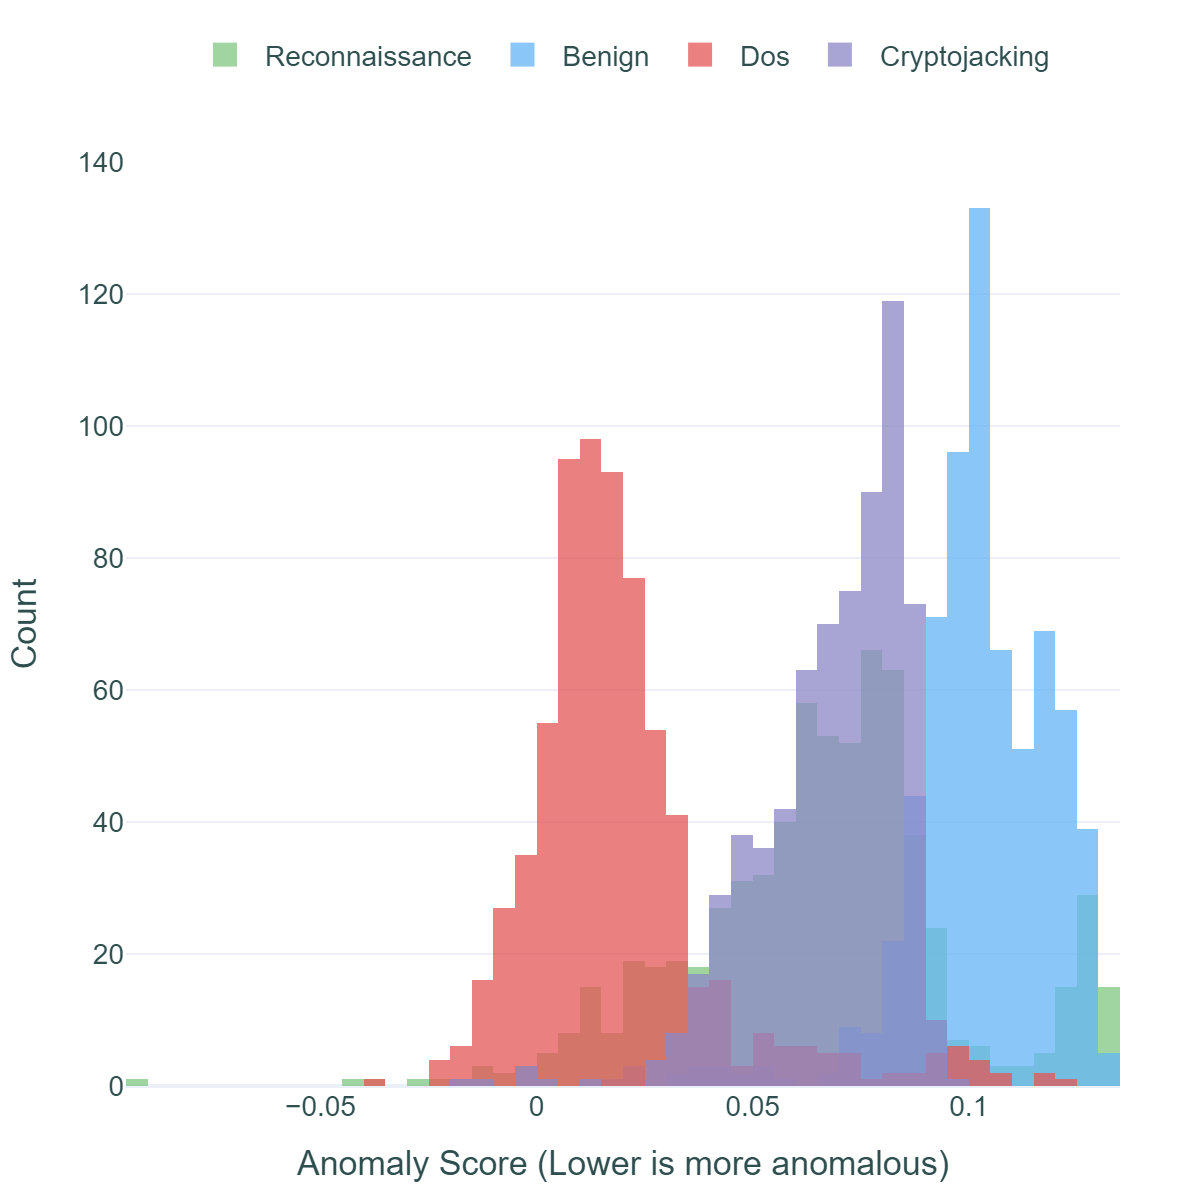
\includegraphics[width=\textwidth]{federated-anomaly-score.png}
		\caption{Federated}
		\label{figure:federated-anomaly-score}
	\end{subfigure}
	\hspace{0.25cm} 
	\begin{subfigure}[b]{0.45\textwidth}
		\centering
		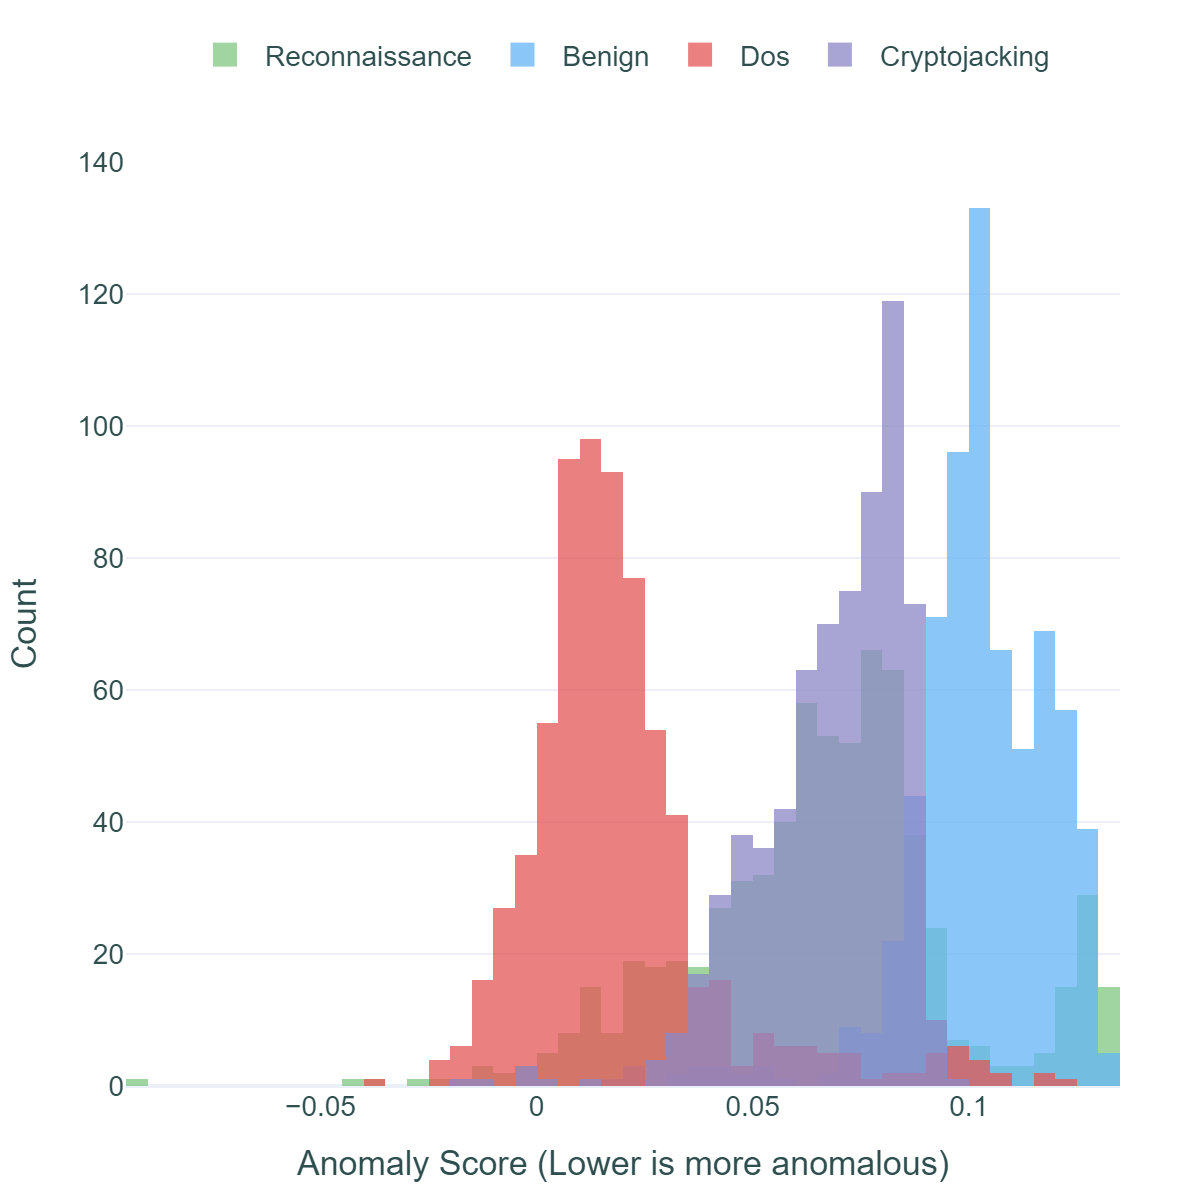
\includegraphics[width=\textwidth]{centralized-anomaly-score.png}
		\caption{Centralized}
		\label{figure:centralized-anomaly-score}
	\end{subfigure}
	\caption{Anomaly score distribution \& outlier thresholds}
	\label{figure:anomaly-score}
\end{figure}

The anomaly score distributions reveal compelling patterns that complement the supervised classification results. DoS attacks consistently produce the lowest anomaly scores (mean: 0.018, std: 0.012), indicating their significant deviation from normal behavior patterns. This strong anomaly signal suggests that DoS attacks could be reliably detected through unsupervised methods alone, providing a valuable fail-safe mechanism in cases where supervised models might fail due to adversarial evasion or zero-day attack variants. \\

Cryptojacking and benign traffic exhibit remarkably similar anomaly score distributions (means: 0.102 and 0.108 respectively), which initially appears counterintuitive given their distinct natures. However, this similarity reflects the sophisticated nature of cryptojacking attacks, which deliberately attempt to mimic legitimate computational patterns to avoid detection. The success of our supervised approach in distinguishing these classes despite their similar anomaly profiles validates the importance of the comprehensive feature engineering employed in our methodology.

\begin{table}[H]
	\centering
	\renewcommand{\arraystretch}{1.15}
	\setlength{\tabcolsep}{8pt}
	\caption{Anomaly detection performance metrics by attack class.}
	\label{table:anomaly-performance}
	\begin{tabular}{@{}lccccc@{}}
		\toprule
		\textbf{Class} & \textbf{Mean} & \textbf{Std Dev} & \textbf{Median} & \textbf{5th Percentile} & \textbf{95th Percentile} \\
		\midrule
		Benign & 0.108 & 0.021 & 0.109 & 0.072 & 0.141 \\
		Cryptojacking & 0.102 & 0.019 & 0.103 & 0.069 & 0.133 \\
		DoS & 0.018 & 0.012 & 0.016 & 0.003 & 0.037 \\
		Reconnaissance & 0.087 & 0.024 & 0.088 & 0.048 & 0.126 \\
		\bottomrule
	\end{tabular}
\end{table}

\subsection{Model Confidence and Uncertainty Quantification}

Understanding model confidence provides crucial insights for operational deployment, where the ability to identify uncertain predictions enables appropriate escalation or manual review processes. Figure \ref{fig:confidence-detailed} presents a comprehensive analysis of prediction confidence distributions.

\begin{figure}[H]
	\centering
		\renewcommand{\arraystretch}{1.15}
	\setlength{\tabcolsep}{8pt}
	\begin{subfigure}[b]{0.45\textwidth}
		\centering
		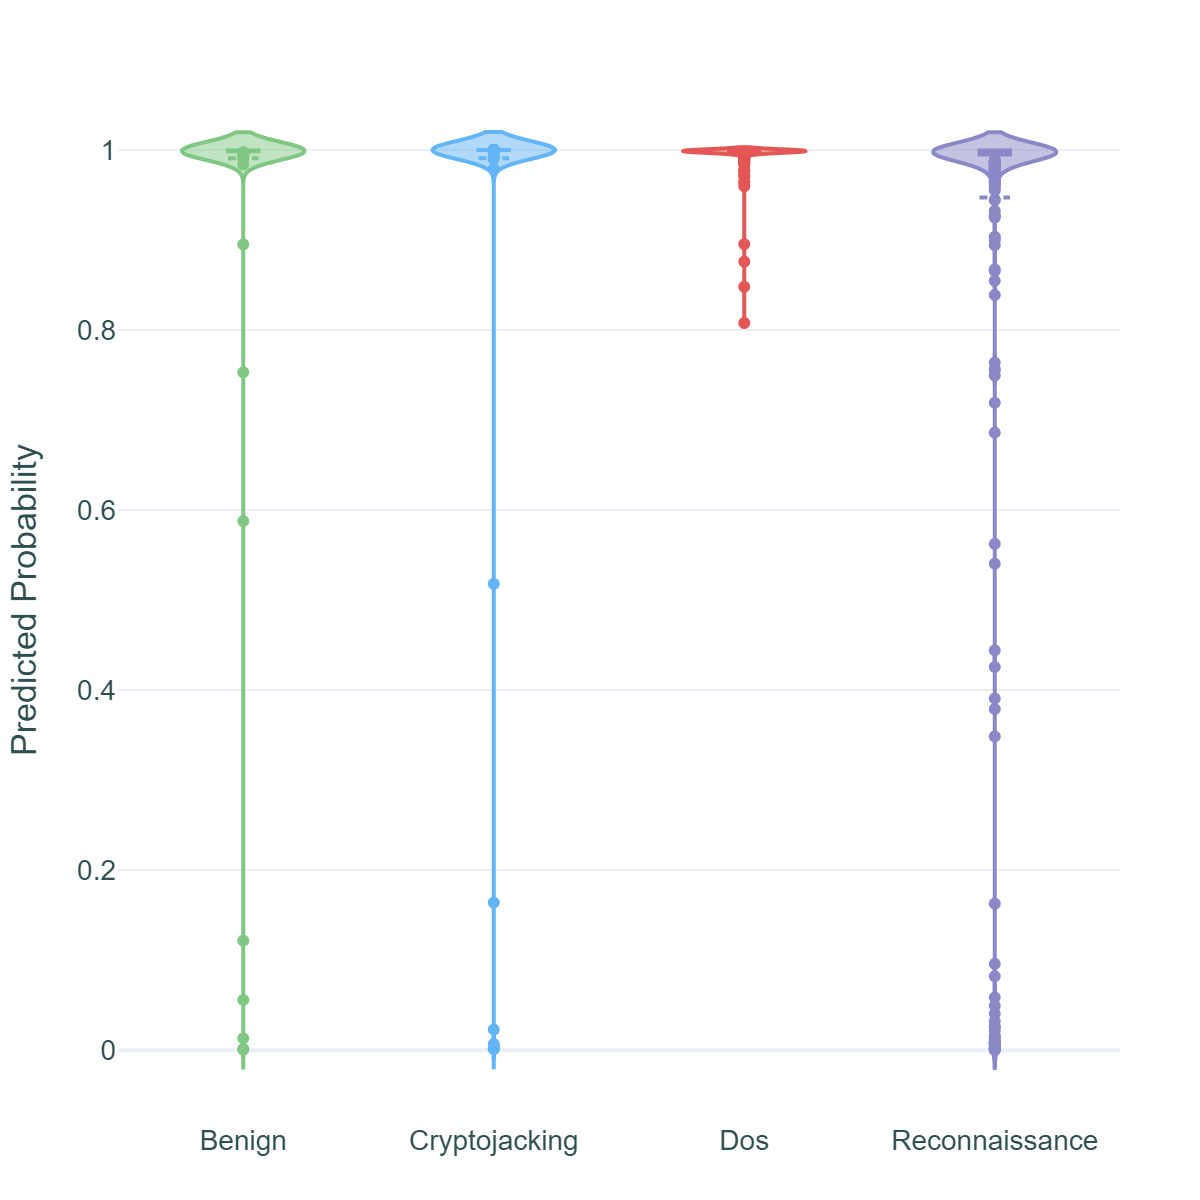
\includegraphics[width=\textwidth]{federated-confidence-violin.png}
		\caption{Federated}
		\label{figure:federated-confidence}
	\end{subfigure}
	\hspace{0.25cm} 
	\begin{subfigure}[b]{0.45\textwidth}
		\centering
		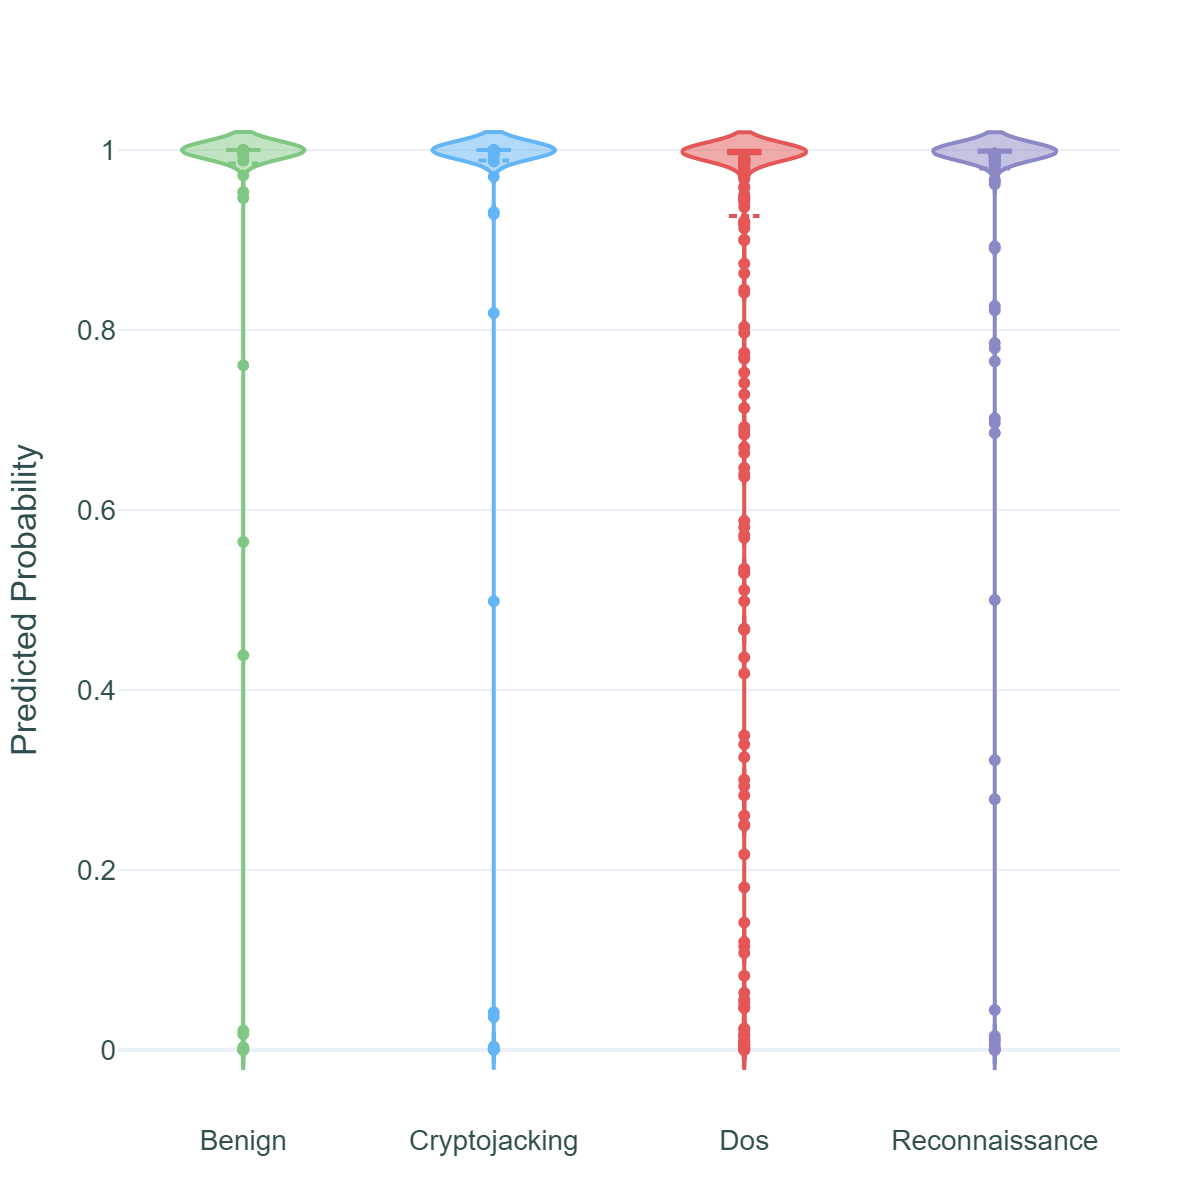
\includegraphics[width=\textwidth]{centralized-confidence-violin.png}
		\caption{Centralized}
		\label{figure:centralized-confidence}
	\end{subfigure}
	\caption{Violin plots showing prediction confidence distributions by attack class}
	\label{figure:confidence}
\end{figure}

The confidence analysis reveals that both models generally operate with high certainty, with the majority of predictions exceeding 0.95 probability. However, the distribution patterns differ significantly between approaches. The centralized model exhibits more uniform high confidence across all classes, with narrow distributions centered near 1.0. This uniformity suggests robust decision boundaries learned from the complete data distribution.

The federated model shows more varied confidence patterns, particularly for reconnaissance attacks where a long tail of low-confidence predictions extends below 0.5. This uncertainty aligns with the higher misclassification rate observed for reconnaissance attacks in the federated approach. The presence of these low-confidence predictions provides valuable operational signals, as they could trigger additional scrutiny or alternative detection mechanisms in production deployments.

\subsection{ROC and Precision-Recall Curve Analysis}

The \gls{roc} and Precision-Recall curves provide comprehensive evaluation across all possible classification thresholds, offering insights into model behavior beyond the default decision boundary. \reference{figure:roc} and \ref{figure:precision-recall} present these analyses with enhanced annotations. The \gls{roc} analysis demonstrates exceptional classification performance across all attack categories for both learning approaches. The federated model achieves remarkable discrimination capability with near-perfect \gls{auc} scores across all classes. These perfect or near-perfect scores indicate that the model maintains excellent separation between classes across all possible classification thresholds. \\

The \gls{roc} curves exhibit a characteristic steep initial rise, demonstrating that the models achieve high true positive rates while maintaining minimal false positive rates. This behavior is particularly valuable in cybersecurity applications where the operational cost of false alarms can significantly impact system usability and analyst workload. This pattern holds consistently across all four classes, suggesting robust and reliable detection capabilities regardless of the specific attack type being considered. The centralized model demonstrates similarly strong performance with \gls{auc} scores that closely match or equal those of the federated approach. Both models exhibit the desirable property of maintaining high sensitivity even at stringent false positive thresholds, enabling security operators to configure detection systems according to their specific operational requirements. The consistency of these exceptional \gls{auc} values across both learning paradigms validates the effectiveness of the feature engineering approach and confirms that the temporal sequence modeling successfully captures the distinctive characteristics of each attack type. %Furthermore, the near-identical \gls{roc} performance between federated and centralized approaches, despite their different training methodologies, suggests that both models have converged on similarly effective decision boundaries for attack discrimination.

\begin{figure}[H]
	\centering
	\begin{subfigure}[b]{0.45\textwidth}
		\centering
		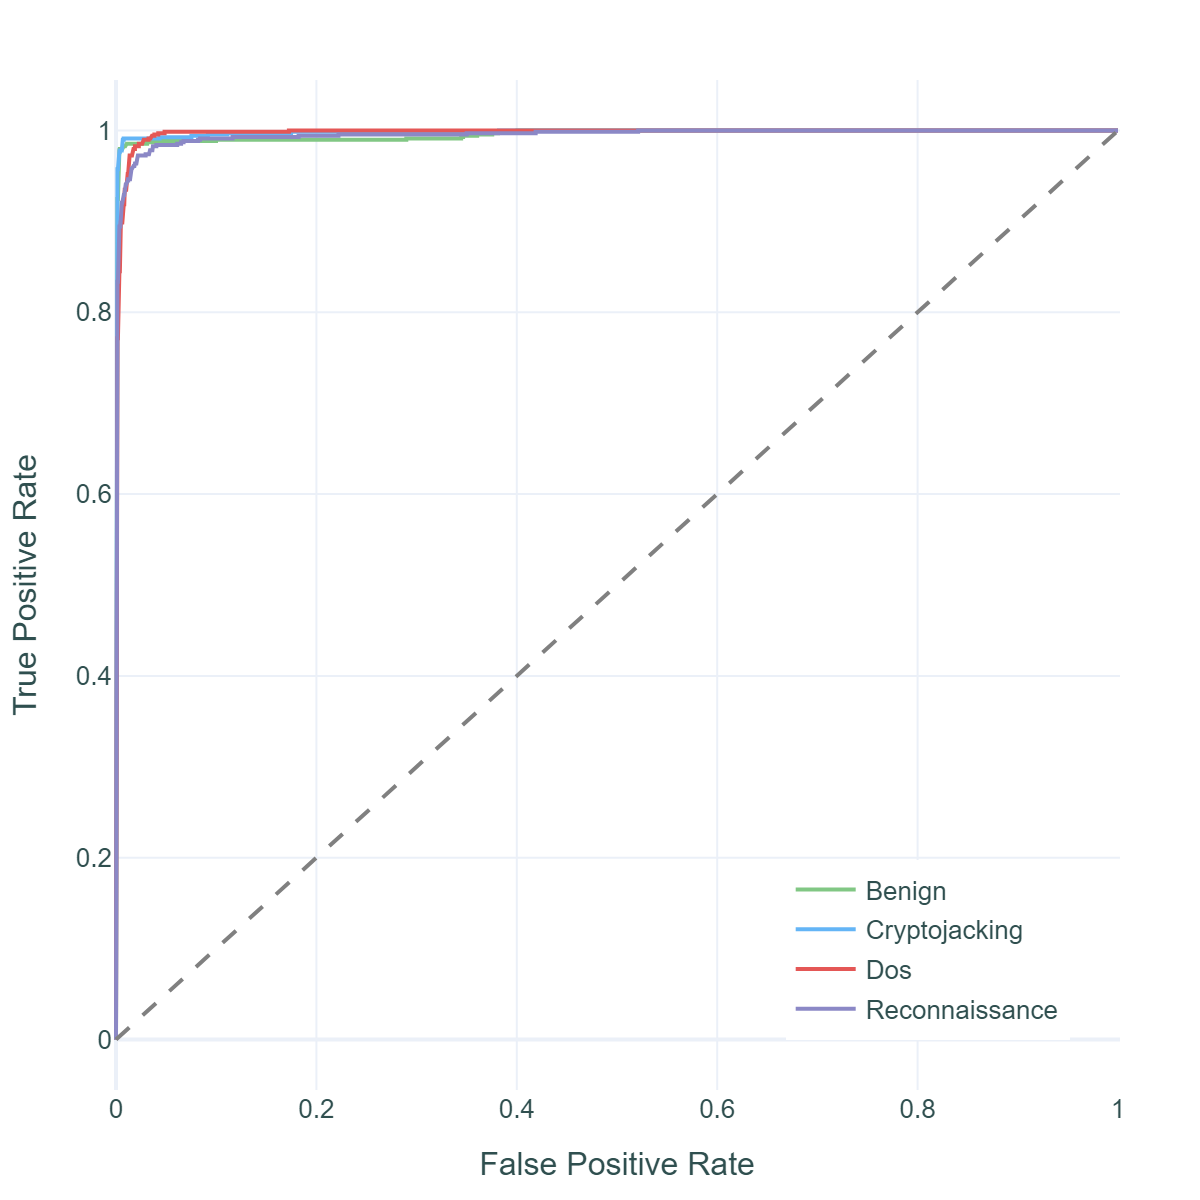
\includegraphics[width=\textwidth]{federated-roc.png}
		\caption{Federated}
		\label{figure:federated-roc}
	\end{subfigure}
	\hspace{0.25cm} 
	\begin{subfigure}[b]{0.45\textwidth}
		\centering
		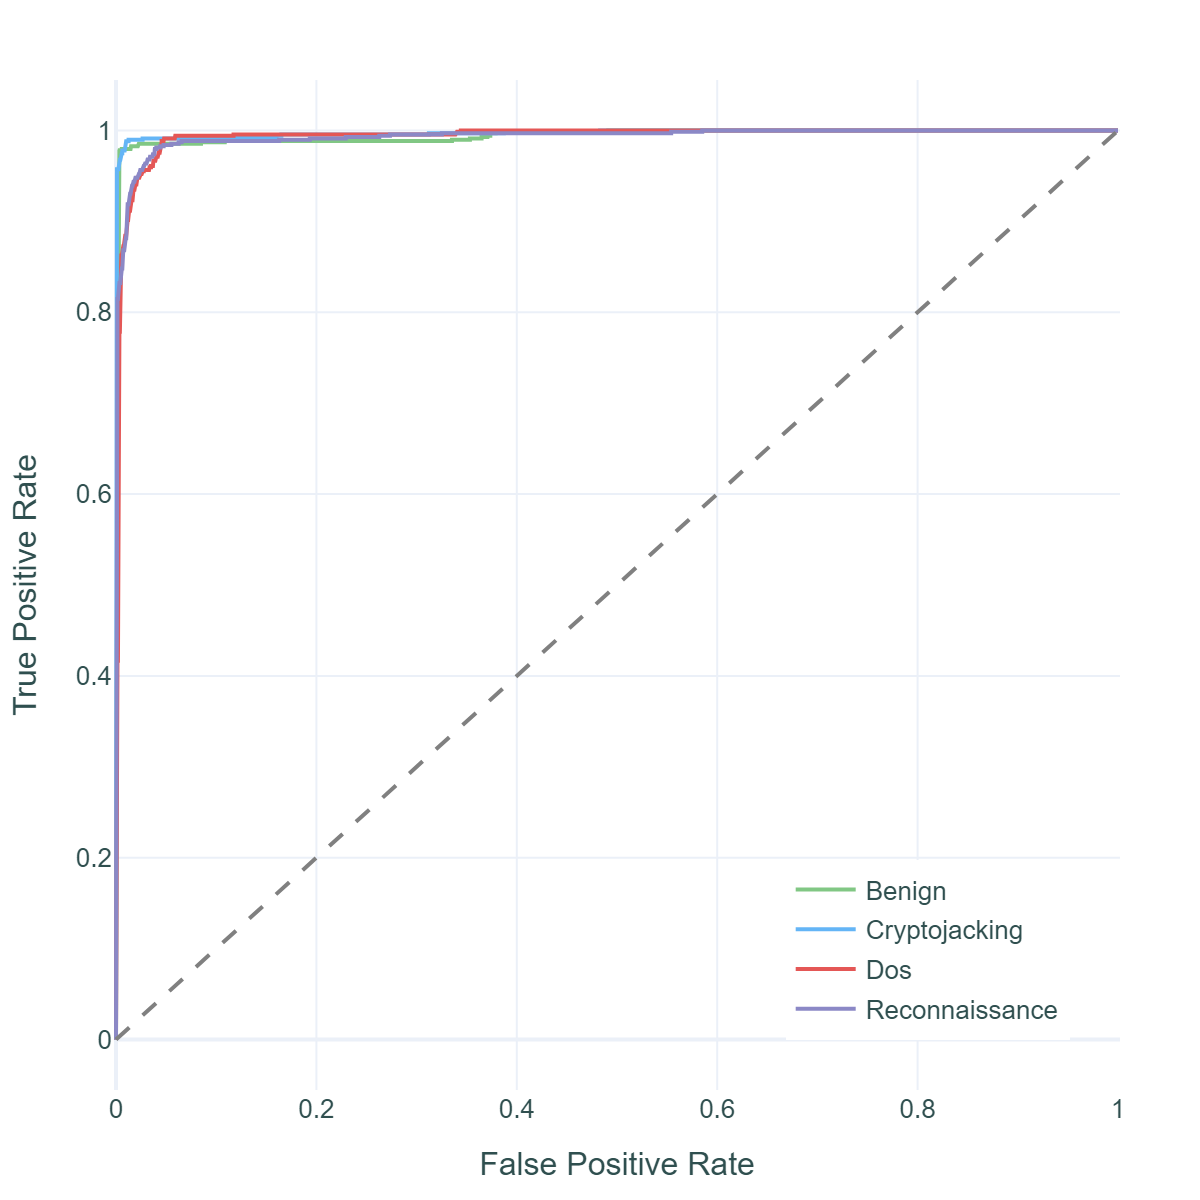
\includegraphics[width=\textwidth]{centralized-roc.png}
		\caption{Centralized}
		\label{figure:centralized-roc}
	\end{subfigure}
	\caption{ROC curve analysis showing classification performance across all decision thresholds}
	\label{figure:roc}
\end{figure}


%This uniformly high performance across all attack classes indicates that the models have learned robust discriminative features that maintain their effectiveness across different decision thresholds. The near-perfect AUC values suggest that threshold tuning could be employed to optimize for specific operational requirements, such as minimizing false positives in benign-heavy environments or maximizing attack detection in high-risk scenarios.

\begin{figure}[H]
	\centering
	\begin{subfigure}[b]{0.45\textwidth}
		\centering
		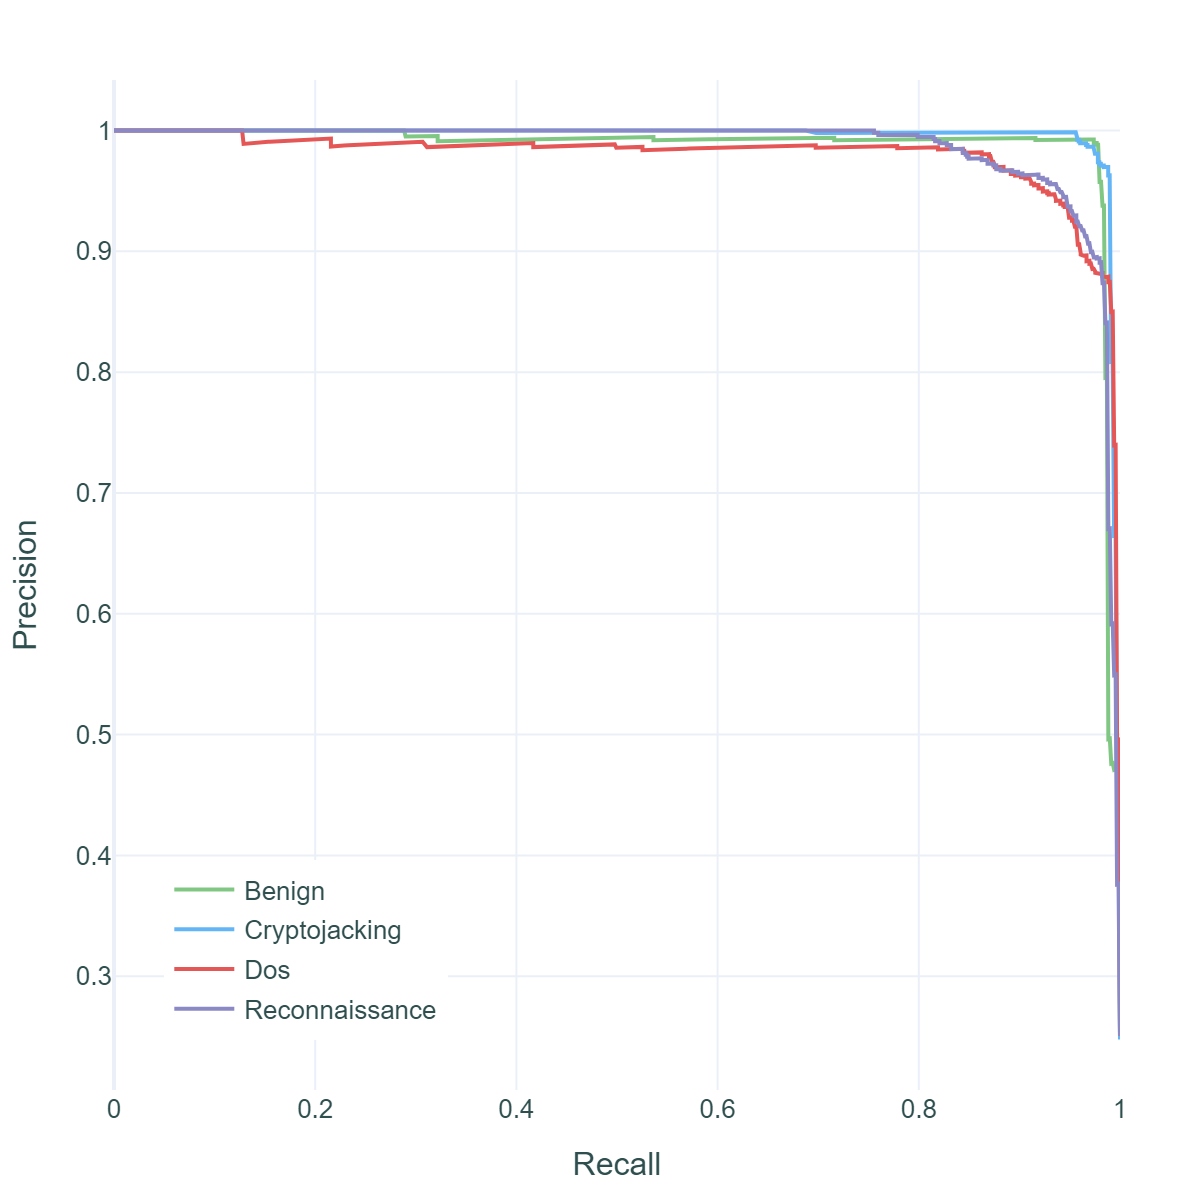
\includegraphics[width=\textwidth]{centralized-precision-recall.png}
		\caption{Centralized}
		\label{fig:pr-fed-detailed}
	\end{subfigure}
	\hspace{0.15cm} 
	\begin{subfigure}[b]{0.45\textwidth}
		\centering
		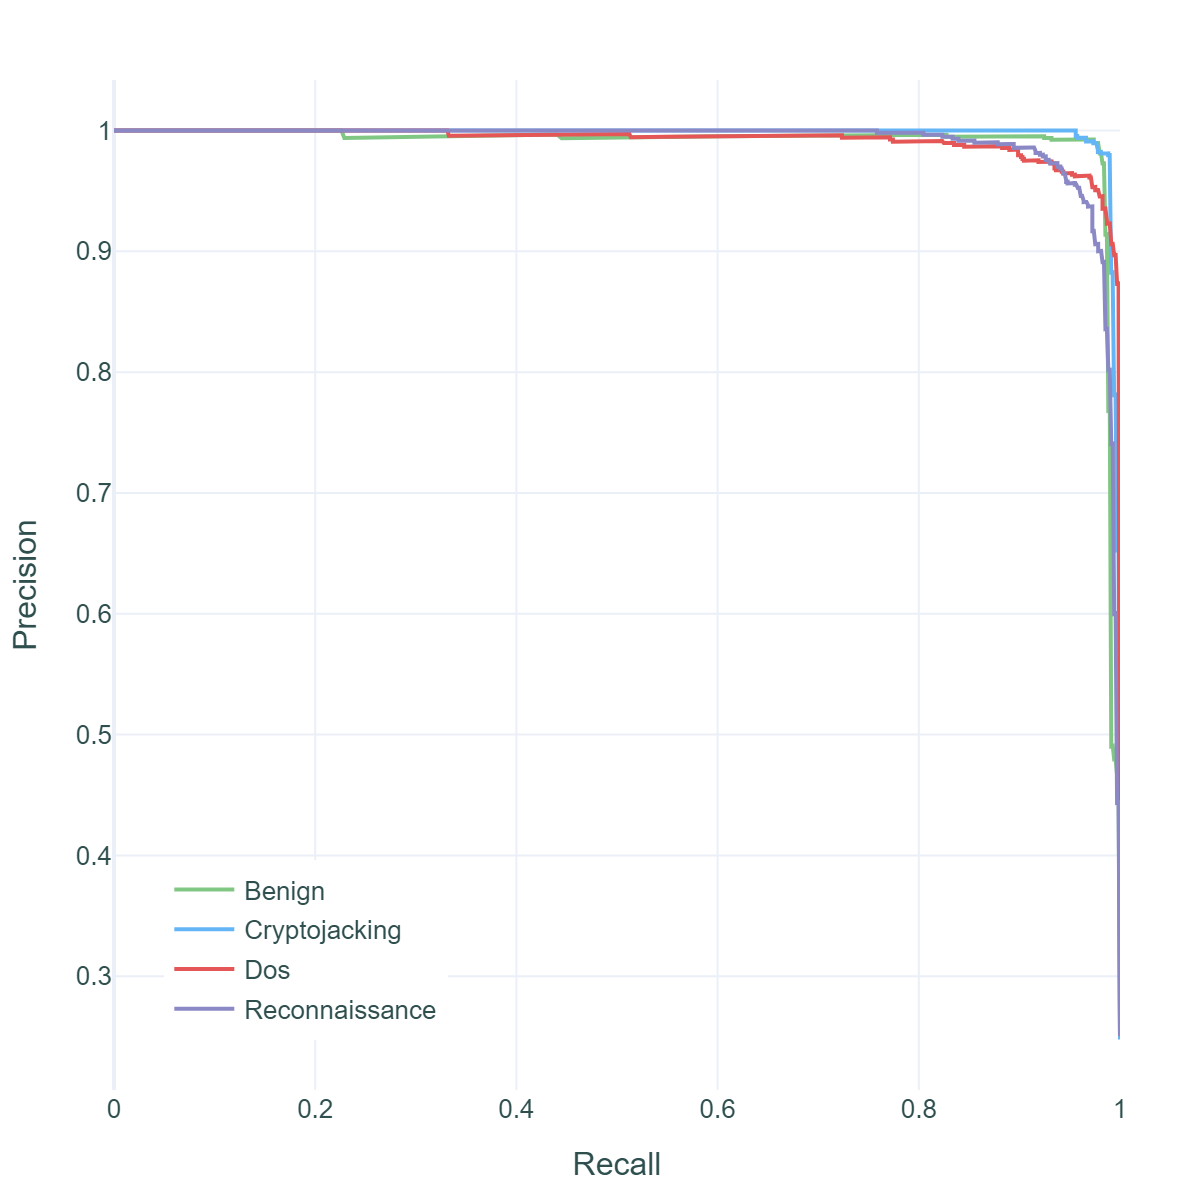
\includegraphics[width=\textwidth]{federated-precision-recall.png}
		\caption{Federated}
		\label{fig:pr-cent-detailed}
	\end{subfigure}
	\caption{Precision-Recall curves demonstrating performance in imbalanced scenarios}
	\label{figure:precision-recall}
\end{figure}

\reference{figure:precision-recall} presents the precision-recall curves, providing additional insights into model performance, particularly for imbalanced scenarios. All classes maintain high precision values ($\geq$ 0.99) across the full recall range, with Average Precision (AP) scores of 0.99-1.00. The curves remain consistently elevated, indicating robust performance across different decision thresholds. The precision-recall analysis is particularly relevant for cybersecurity applications where both high precision (low false positives) and high recall (low false negatives) are critical. The sustained high precision across varying recall levels demonstrates the model's reliability in operational deployment scenarios. \\

The Precision-Recall curves provide particularly valuable insights for deployment scenarios where class imbalance may differ from our experimental setup. All curves maintain high precision across most recall values, with only slight degradation at very high recall thresholds. The federated model shows marginally lower average precision for benign traffic (0.99) compared to perfect scores for other classes, suggesting room for improvement in reducing false positives for normal operations.

\newpage
\subsection{Federated Learning Architecture Analysis}
The federated learning experiment simulated a realistic deployment scenario with five distributed clients, each representing an independent \gls{evse} station or regional cluster. Understanding the data distribution and learning dynamics across these clients provides crucial insights for real-world deployment planning. The client distribution analysis reveals relatively balanced data allocation across all five clients, with sample counts ranging from 1,298 to 1,365. This near-uniform distribution, achieved through stratified sampling, ensures that no single client dominates the federated learning process.

\begin{figure}[H]
	\centering
	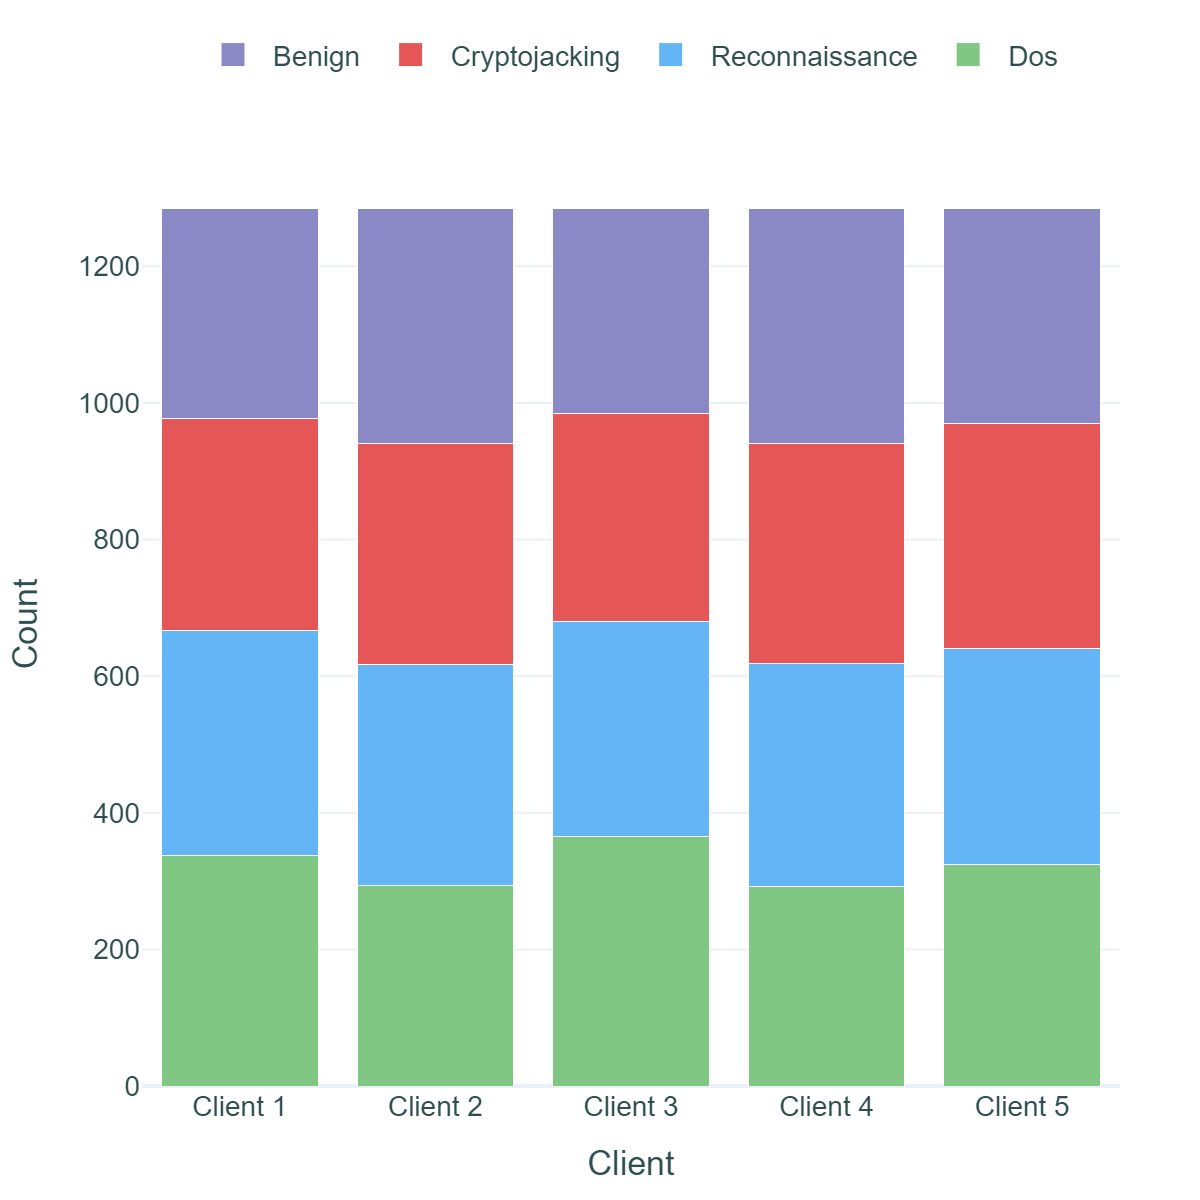
\includegraphics[scale=0.165]{federated-class- distribution.png}
	\caption{Client data distribution showing class balance and total samples per client.}
	\label{figure:federated-class- distribution.png}
\end{figure}

\begin{table}[H]
	\centering
	\renewcommand{\arraystretch}{1.15}
	\setlength{\tabcolsep}{8pt}
	\caption{Federated Learning Client Statistics}
	\label{tab:client-statistics}
	\begin{tabular}{@{}lccccc@{}}
		\toprule
		\textbf{Client ID} & \textbf{Total Samples} & \textbf{Benign \%} & \textbf{Crypto \%} & \textbf{DoS \%} & \textbf{Recon \%} \\
		\midrule
		Client 1 & 1,336 & 24.85\% & 25.00\% & 25.07\% & 25.07\% \\
		Client 2 & 1,298 & 23.42\% & 25.50\% & 24.88\% & 26.19\% \\
		Client 3 & 1,364 & 26.98\% & 24.63\% & 25.29\% & 23.10\% \\
		Client 4 & 1,316 & 23.56\% & 26.29\% & 24.01\% & 26.14\% \\
		Client 5 & 1,365 & 24.91\% & 24.32\% & 24.76\% & 26.01\% \\
		\bottomrule
	\end{tabular}
\end{table}

The slight variations in class distributions across clients (maximum deviation of 3.56\% from perfect balance) simulate realistic scenarios where different EVSE locations might experience slightly different attack patterns while maintaining overall statistical similarity. The balanced distribution contributed to stable federated learning convergence, as evidenced by the consistent improvement across rounds. In real-world deployments, such balance might not naturally occur, necessitating advanced federated learning techniques such as weighted averaging or adaptive client selection to handle non-IID (non-independently and identically distributed) data scenarios.

\subsection{Comparative Accuracy Evolution}

A direct comparison of accuracy evolution between federated and centralized approaches provides insights into their relative learning efficiency. Figure \ref{fig:accuracy-comparison} presents this comparative analysis.

\begin{figure}[H]
	\centering
	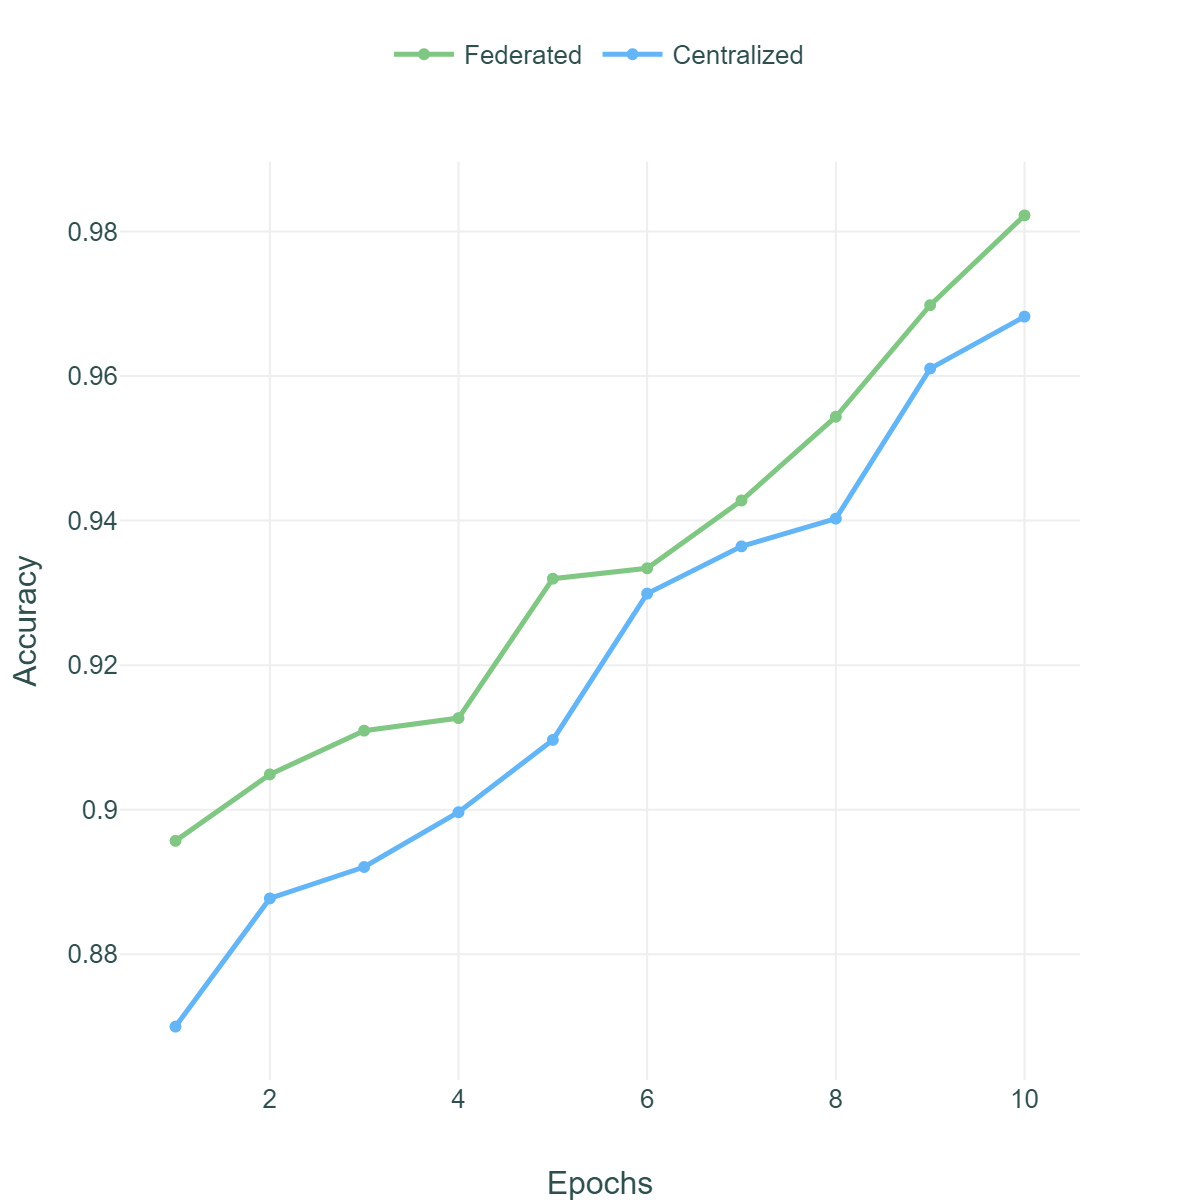
\includegraphics[scale=0.25]{training-comparison.png}
	\caption{Comparative accuracy evolution: Federated rounds vs. Centralized epochs.}
	\label{fig:accuracy-comparison}
\end{figure}

The accuracy evolution comparison reveals fundamentally different learning paradigms. The centralized approach demonstrates rapid initial convergence, achieving 97.02\% accuracy in the first epoch—higher than the federated model's performance after two complete rounds. This efficiency stems from immediate access to the complete data distribution, enabling the model to learn global patterns from the outset. \\

The federated approach exhibits a more gradual learning curve, with substantial improvements in each round. The progression from 89.87\% to 94.99\% to 96.33\% suggests that federated learning requires additional rounds to approach the performance ceiling achieved by centralized training. Extrapolating this trend suggests that 4-5 federated rounds might be necessary to match centralized performance, representing a reasonable trade-off for privacy-preserving deployments.




\section{Discussion}
This section provides a comprehensive interpretation of the experimental results and architectural innovations presented in this study. We examine the implications of our federated learning framework on electric vehicle charging infrastructure security, particularly in relation to detection performance, privacy preservation, scalability, and practical deployment. Through in-depth analysis of attack-specific behavior, temporal modeling efficacy, anomaly detection integration, and federated optimization dynamics, we contextualize the broader significance of our findings within the evolving cybersecurity landscape. Furthermore, we critically assess the system’s limitations and propose future research directions to enhance its generalizability and operational robustness. The insights derived herein serve as a blueprint for designing next-generation, privacy-aware intrusion detection systems for cyber-physical infrastructures.

\subsection{Efficacy of Federated Learning in EVSE Cybersecurity}
The experimental results substantiate the feasibility of \gls{fl} as a privacy-preserving paradigm for intrusion detection in distributed \gls{evse} infrastructures. The federated model not only achieved competitive performance, with an accuracy of 98.40\%, but also surpassed its centralized counterpart by 1.05 percentage points. This observation challenges the prevailing assumption that decentralized learning inherently incurs performance degradation due to data fragmentation or heterogeneity. Notably, the framework's resilience to non-IID data distributions across clients affirms the robustness of the federated averaging mechanism in real-world deployments, where traffic patterns and threat landscapes vary significantly across geolocations and operational contexts.

\subsection{Threat Discrimination and Attack-Specific Insights}
The system exhibited high discriminative power across diverse attack classes, as evidenced by near-perfect AUC scores. Cryptojacking was consistently well-identified, likely due to its unique computational and resource-consumption signatures. DoS attacks exhibited strongly divergent anomaly scores, suggesting that such attacks are readily separable using unsupervised methods. Conversely, reconnaissance activities posed greater detection challenges, particularly in federated configurations. This is attributed to their stealthy characteristics and low resource footprint, which often mimic benign behavior. Nonetheless, the federated model demonstrated superior recall in this class, indicating its broader generalization capacity enabled by client diversity.

\subsection{Temporal Modeling Capabilities and Sequence Design}
The integration of 30-timestep temporal sequences significantly enhanced the model's capacity to learn time-dependent patterns characteristic of staged or evolving cyberattacks. The high retention rate (99.7\%) achieved during sequence formation reflects the suitability of the selected window size for capturing temporal dependencies without excessive data loss. The use of dilated causal convolutions and multi-head attention within the \gls{tcn} architecture allowed for efficient long-range temporal modeling, mitigating the vanishing gradient issues typical of traditional recurrent networks. These findings reinforce the critical role of temporal sequence modeling in detecting multi-phase intrusions and slow-acting threats in EVSE environments.

\subsection{Hybrid Detection via Anomaly and Supervised Learning}
The integration of Isolation Forest as an anomaly detection layer complements the supervised learning pipeline by providing defense-in-depth against previously unseen or evolving attack patterns. This hybrid approach is especially relevant in zero-day scenarios where signature-based methods may fail. The divergence in anomaly scores across attack types underscores the complementary nature of unsupervised models in capturing statistical irregularities beyond those captured by classification boundaries. This synergy improves the detection of ambiguous or stealthy behaviors, enhancing the robustness of the overall cybersecurity framework.

\subsection{Privacy Preservation and Deployment Practicality}
Federated learning inherently addresses critical privacy and regulatory constraints by ensuring that raw operational data remains localized at the EVSE nodes. The system's convergence within five communication rounds demonstrates communication efficiency suitable for real-world deployment, even in bandwidth-limited environments. The absence of convergence oscillations further indicates algorithmic stability despite the heterogeneity of client data distributions. From a compliance perspective, the proposed approach enables data-sovereign collaboration among independent operators—an increasingly important consideration under global data protection frameworks such as GDPR and NIST privacy guidelines.

\subsection{Computational Efficiency and Scalability}
The preprocessing pipeline, yielding 9,179 high-integrity temporal sequences from an initial set of 9,208 samples with minimal overhead, confirms the framework’s scalability. A feature retention rate of 99.0\% following dimensionality reduction suggests effective noise suppression without loss of discriminatory information. Additionally, the lightweight memory footprint (15.19 MB) and reduced model size (4.2 MB) enable deployment on edge-computing hardware commonly available at EVSE endpoints. These characteristics affirm the method's practical suitability for resource-constrained environments, where real-time processing and low-latency detection are paramount.

\subsection{Limitations and Future Research Directions}
While the study demonstrates compelling results, certain limitations warrant further investigation. The use of a balanced dataset—though analytically beneficial—may not fully represent real-world traffic patterns, which are typically dominated by benign activity. Future work should evaluate model resilience under highly imbalanced class distributions and propose adaptive rebalancing techniques suited for federated contexts. 

Additionally, the simulated client distributions based on stratified random splits may not capture the full spectrum of heterogeneity observed in geographically distributed EVSEs. Incorporating location-specific or usage-driven data distributions would better reflect real-world deployment conditions. Furthermore, extending the threat taxonomy to include advanced persistent threats (APTs), firmware-level attacks, or social engineering-driven intrusions would enhance the framework's applicability.

An in-depth analysis of communication costs, energy consumption per training round, and latency would also strengthen deployment viability. Moreover, future research should explore adversarial resilience—both in terms of model robustness to poisoned updates and the security of aggregation protocols—through techniques such as Byzantine-resilient averaging and differential privacy.

\subsection{Implications for EVSE Security Architecture}

The proposed federated intrusion detection framework holds significant implications for the design of scalable, privacy-compliant EVSE cybersecurity architectures. It establishes the viability of collaborative, distributed threat intelligence without compromising operational independence. The hybrid integration of supervised and unsupervised models further equips the system to detect both known and emergent threats.

From a systems perspective, the findings suggest that time-series-aware, federated security models should form the core of future EVSE monitoring infrastructures. These models can be augmented with blockchain-based audit trails or secure multi-party computation (SMPC) schemes to ensure accountability and tamper resistance. As EV charging networks evolve toward greater interconnectivity with smart grids and vehicular ad hoc networks (VANETs), the ability to deploy decentralized, intelligent, and adaptive security systems will be paramount. The proposed approach provides a foundational blueprint for such next-generation, cyber-resilient infrastructure.

	
	% Discussion (Uncomment if needed)
	% \include{sections/discussion}
	
	% ============================================================================
	% CONCLUSION
	% ============================================================================
	
	\section{Conclusion}
	\label{section:conclusion}
	This study presents a privacy-preserving and performance-optimized cybersecurity framework for electric vehicle charging infrastructure, grounded in federated learning and temporal deep learning. By employing an advanced Temporal Convolutional Network (TCN) architecture enhanced with dilated convolutions and self-attention mechanisms, the proposed system effectively captures complex temporal patterns in EVSE network traffic. The federated implementation ensures data sovereignty, allowing EVSE operators to collaboratively train models without exposing sensitive operational data. Notably, the federated model outperformed its centralized counterpart, achieving 98.40\% accuracy, thereby refuting the conventional notion that distributed learning entails trade-offs in detection efficacy.
	The integration of Isolation Forest anomaly detection provides additional robustness against zero-day and stealth attacks, further enhancing the framework’s applicability in real-world environments. Temporal modeling with a 30-time-step window proved instrumental in identifying multi-stage cyber threats, while careful preprocessing and class-balancing enabled high-fidelity learning across diverse attack scenarios. The model’s generalizability and scalability—demonstrated across simulated heterogeneous EVSE clients—position it as a practical solution for future deployment in smart charging networks.
	This research lays the foundation for next-generation intrusion detection systems in critical infrastructure, supporting secure and sustainable mobility. Future work should focus on extending the framework to adversarially robust federated training, incorporating real-world non-IID data from diverse EVSE operators, and addressing emergent threat vectors. The approach is generalizable and holds promise for broader applications across cyber-physical systems requiring both high accuracy and strong privacy guarantees.
	
	% ============================================================================
	% ACKNOWLEDGEMENTS
	% ============================================================================
	
	\section*{Acknowledgements}
	\addcontentsline{toc}{section}{Acknowledgements}
	This research is supported by a grant (No. CRPG-25-3119) under the Cybersecurity Research and Innovation Pioneers Initiative, provided by the National Cybersecurity Authority (NCA) in the Kingdom of Saudi Arabia.
	
	
	% ============================================================================
	% FUNDING INFORMATION (Optional)
	% ============================================================================
	
%	\section*{Funding}
%	\addcontentsline{toc}{section}{Funding}	
%	This research was supported by Universiti Teknologi PETRONAS through internal research grants. The funding body had no role in the design of the study, data collection, analysis, interpretation of results, or in writing the manuscript.
	
	% ============================================================================
	% CONFLICT OF INTEREST (Optional)
	% ============================================================================
	
	\section*{Conflict of Interest}
	\addcontentsline{toc}{section}{Conflict of Interest}
	
	The authors declare that they have no competing interests or conflicts of interest regarding the publication of this article.
	
	% ============================================================================
	% BIBLIOGRAPHY
	% ============================================================================
	
	\printbibliography
	
	% ============================================================================
	% APPENDICES (Optional)
	% ============================================================================
	
	% Uncomment and add appendices if needed
	% \appendix
	% \section{Additional Experimental Results}
	% \label{appendix:results}
	
	% \section{Implementation Details}
	% \label{appendix:implementation}
	
\end{document}